%% 
%% Copyright 2007-2020 Elsevier Ltd
%% 
%% This file is part of the 'Elsarticle Bundle'.
%% ---------------------------------------------
%% 
%% It may be distributed under the conditions of the LaTeX Project Public
%% License, either version 1.2 of this license or (at your option) any
%% later version.  The latest version of this license is in
%%    http://www.latex-project.org/lppl.txt
%% and version 1.2 or later is part of all distributions of LaTeX
%% version 1999/12/01 or later.
%% 
%% The list of all files belonging to the 'Elsarticle Bundle' is
%% given in the file `manifest.txt'.
%% 
%% Template article for Elsevier's document class `elsarticle'
%% with harvard style bibliographic references

\documentclass[final,5p,times,twocolumn]{elsarticle}

%% Use the options 1p,twocolumn; 3p; 3p,twocolumn; 5p; or 5p,twocolumn
%% for a journal layout:
%% \documentclass[final,1p,times]{elsarticle}
%% \documentclass[final,1p,times,twocolumn]{elsarticle}
%% \documentclass[final,3p,times]{elsarticle}
%% \documentclass[final,3p,times,twocolumn]{elsarticle}
%% \documentclass[final,5p,times]{elsarticle}
%% \documentclass[final,5p,times,twocolumn]{elsarticle}

%% For including figures, graphicx.sty has been loaded in
%% elsarticle.cls. If you prefer to use the old commands
%% please give \usepackage{epsfig}

%% The amssymb package provides various useful mathematical symbols
\usepackage[utf8]{inputenc}
\usepackage{textcomp}

\usepackage{graphicx}
\usepackage{float}

\usepackage{times}
\usepackage{color}
\usepackage{xcolor}
\usepackage{natbib} 
\usepackage{enumerate}
\usepackage{caption}
%\usepackage[separator = {;}]{credits}
\usepackage{lscape}
\usepackage{subcaption}
\usepackage{wrapfig}
\usepackage{orcidlink}
\usepackage{amssymb}
\usepackage{amsthm}
\usepackage{enumitem}
\usepackage{hyperref}
\hypersetup{colorlinks=true,
	 citecolor=cyan,
	 pdfauthor=cyan,
	 linkcolor=cyan}


\journal{Journal of Optics and Laser in Engineering}

\begin{document}

\begin{frontmatter}

\title{Small Satellite Electro-Optical System(EOS) Technological and Commercial Expansion}
\tnotetext[t1]{This document is the results of the research project funded by the Aerospace System and Control Lab, ASCL}

\author[1]{Gadisa Dianol\corref{cor1}}
\fnref{fn1}
\ead{gdina@kaist.ac.kr}
%\credit{Conceptualization,  Writing - Original draft, Methodology, Data curation, Writing -review and editing, and Visualization }
\author[1]{Hyochoong Bang\fnref{fn2}}
\ead{hcbnag@kaist.ac.kr}
%\credit{Reviewing and editing,  Supervision, and Funding acquisition}
\cortext[cor1]{Corresponding author}
\fntext[fn1]{Researcher at Aerospace System and Control Lab, Department Aerospace engineering, KAIST, 34141, Republic of Korea}
\fntext[fn2]{Professor of Aerospace Engineering at Korean Advanced Institute of Science and Technology (KAIST), Daejeon, 34141, Republic of Korea}

\affiliation[1]{organization={Aerospace System and Control Lab, Korean Advanced Institute of Science and Technology, KAIST},%Department and Organization
            addressline={291}, 
            city={Daejoen},
            postcode={34141}, 
            country={Republic of Korea}}
%\affiliation[2]{}
\begin{abstract}
The use of electro-optical imaging system for commercial, military, or surveillance missions, as well as space scientific missions, dates back to the first successful operation aboard the US Explorer-6 spacecraft, which was the first spacecraft to capture low-resolution images of the Earth's surface, and the Luna-3 space probe, which was the first spacecraft to send images of the lunar far side, in 1959. The technology underlying EO system have evolved over time, with advances in optics, electronics, and materials science leading to the development of more sophisticated and capable imaging sensors. Furthermore, the technological advances in sensors, optics, mechanics, material, signal and image processing algorithms have allowed EO payloads to become smaller, lighter, and more efficient while still providing high-quality imagery.
Over 840 small spacecraft weighing less than 500 kg were launched, with 80\% in the constellation segment and 20\% as monolithic satellites (i.e., single spacecraft equipped with an electro-optical imaging instrument launched into space for various missions). In this paper, the electro-optical imaging systems of these spacecraft were examined using data from a variety of sources, including peer-reviewed journal publications, conference proceedings, mission webpages, and other publicly available satellite databases. 
Furthermore, the technological and commercial expansion of small spacecraft ($<$ 500 kg) equipped with electro-optical imaging systems, as well as EO-COTS parametric performance values including GSD, spectral range, field of view, SNR, data storage and transmission rate through 2023 are presented, divided by spacecraft types: SSO satellites, deep space spacecraft, and EO commercialization.
\end{abstract}

%%Research highlights
%\begin{highlights}
%\item Optical sensors and instruments were tuned to acquire black and white images of Earth
%\item Evolution of electro-optical imaging system
%\item Improvement and advancement of electro-optical imaging system
%\item Growing demand for high quality imagery data
%\item Electro-optical based spacecraft in various orbital regimes
%\item Small satellites such as mini-satellites, microsatellites, and nanosatellites
%\item Growing technological and commercial expansion of electro-optical systems of small satellites
%\end{highlights}

\begin{keyword}
	CubeSat \sep Commercial-off-the-shelf (COTS) \sep  Electro-optical \sep Optical imaging  \sep  FoV \sep GSD\sep Small spacecraft \sep  SNR \sep  Sensor 

\end{keyword}
\end{frontmatter}


%% main text
\section{Introduction}
\label{}
The evolution of electro-optical imaging systems can be traced back to the early days of space rivalry in the 1950s. In 1959, the United States launched the first successful reconnaissance satellite, CORONA (KH-4B) (Fig. 2), which carried a TV camera system capable of capturing images of the Earth's surface \citep{ruffner1995corona}, and the US's Explorer-6 spacecraft returned the first TV images from space \citep{christopherson20192019, judge1962observations}, ushering in the use of electro-optical sensors in space reconnaissance, scientific, and intelligence gathering.\\
The development and utilization of electro-optical imaging systems has improved over time, driven by the demands of commercial, military, or surveillance operations, as well as space research missions, as illustrated in Fig. 1. Section 2 also highlights the early phase of optical sensor development and its improvement over time.
\begin{itemize}
	\item \textbf{1st generation}: In the early phase, the optical sensors and instruments were tuned to acquire black and white images of Earth with limited spatial resolution, which were mounted on experimental observational and meteorological satellites that started to fly in the 1960s \citep{nicholas1999} with the TIROS (total of 10) and Nimbus (total of 7) spacecraft series. Other optical sensors on these spacecraft could conduct soundings or observations of atmospheric properties at various heights.
	\item \textbf{2nd generation}: As the demand for an operational system for collecting information about the Earth increased, the development of remote sensing optical imaging continued to improve around the 1970s, when the optical system was flown on the Landsat, first satellite dedicated specifically to monitoring land and ocean surfaces to amp natural and cultural resources. By the 1980s, Landsat had been privatized, and widespread commercial use of remote sensing had taken root in the United States, France, Russia, Japan, and other countries \citep{nicholas1999}. Since the Landsat program's planning and development began with the first launch of Landsat-1, earth observation data have been collected over four decades \citep{wulder2019current} using different optical imaging systems. The Landsat optical imaging system includes a set of sensors and camera's that capture data in the visible, near-infrared, and thermal-infrared regions of the electromagnetic spectrum and it has undergone several upgrades and improvements over the years including the development of Enhanced Thematic mapper Plus (ETM+), which was first launched in 1999 to improve the quality and resolution of the data collected. 
	\item \textbf{3rd generation}: With the introduction of multispectral and hyperspectral imaging systems in the mid-1980s and 1990s, which could capture images in several narrow spectral bands, electro-optical remote sensing imaging systems advanced even further. However, in the late 1990s, a new platform known as CubeSat was launched, which later acknowledged its potential \citep{poghosyan2017cubesat} in deploying multiple payload systems, including optical imaging payload, for diverse applications. Furthermore, these systems provided more spectral detail and enabled a broader range of applications, such as land cover categorization, mineral prospecting, and military reconnaissance. 
	\item \textbf{4th generation}: From 2010 to the present, the technology for electro-optical imaging systems evolved with the introduction of more advanced sensors, such as polarimetric and interferometric imaging systems, and its application has been widely recognized in space missions from space to earth and earth to space, such as the exploration of other planetary bodies \citep{clark2003imaging}. These sensors allowed for the measurement of additional parameters such as surface roughness and terrain elevation, which were useful for a wide range of applications such as geological mapping, disaster response, and land use planning.  And, at the moment, technology for electro-optical remote sensing imaging systems is advancing, with the development of sensors with higher spatial resolution, such as sub-meter resolution, and the incorporation of new technologies, such as synthetic aperture radar (SAR) and lidar, as well as the introduction of new image processing algorithms based on artificial intelligence (AI). 
\end{itemize}
As the demand for high-quality and high-resolution picture data develops, numerous space startups, including SATLANTIS, Planet Lab, Satellogic, Dragonfly Aerospace, Simera Sense, as well as others, are introducing EO-COTS optical sensors solutions of small spacecraft platforms to worldwide markets. These systems are frequently imaging equipment or sensors that capture photographs of the Earth's surface or other planetary bodies for a variety of purposes such as scientific research, remote sensing, and earth observation. Furthermore, they are typically smaller and less expensive than conventional satellite optical payloads and are designed to be used on CubeSats or other small satellite platforms. They frequently use advanced sensors and optics, as well as image processing algorithms, to provide high-quality data and images from space.\\
Overall, the evolution of electro-optical imaging systems mounted on large spacecraft to today's miniaturized small satellite has been fueled by a variety of technological advances and shifting market demands for various sectors such as civil engineering and construction, agriculture and forestry, transportation sectors, and play an important role in space-based applications used by government, military, intelligence, and commercial organizations.\\
A variety of review papers on the use and proliferation of electro-optical technologies deployed with small spacecraft for various application areas can be found in the literature. Nithianandam et al. \citep{JNithianandam_1993} presented an evolution of satellite sensors for Earth observations in the infrared, visible, and ultraviolet spectral regions, as well as a comparison of previous scanning remote sensors and the earth observing system.
Mika \citep{mika1997three} presented the evolution of multispectral sensors for the Landsat series of spacecraft, from the first MSS abroad, Landsat 1, to the most recent version of the Enhanced Thematic mapper for Landsat-7, while Jackson \citep{jackson1997system} described the proposed conceptual design of electro-optical imaging for sea ice from space in the visible and infrared spectra, primarily for surveillance of icebergs and pack ice in northern latitudes. Teleti \citep{teleti2013sea} also discussed the evolution of sensor specifications used for remote sensing in the past and present, with a focus on their suitability for observing polar areas.
Peighani-Asl \citep{peighani2010electro} focused on the optical design process and various factors such as MTF, SNR, FOV, aperture diameter, stability and pointing, scanning schemes, detector selection, and target radiance. Sandau \citep{sandau2010status}, provided the general trends in the field of small satellite missions for earth observation, with particular attention paid to the potential of spectral, spatial, and temporal resolution of small spacecraft's optical payload.  Heo \citep{heo2012design} presented the design and implementation of MAEPLE, a versatile electro-optical camera system for lunar exploration. 
\begin{figure*}
	\centering
	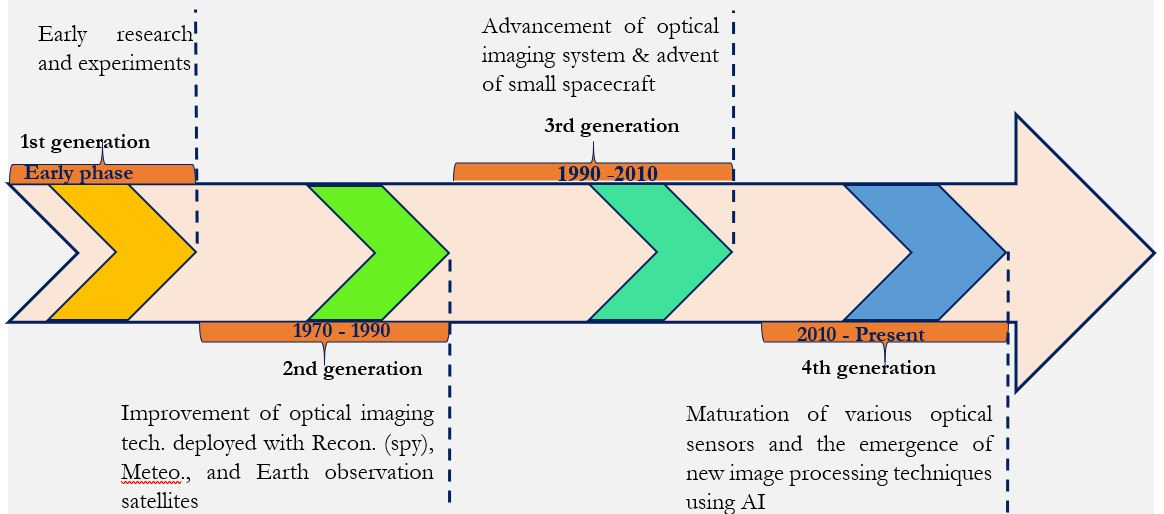
\includegraphics[width=.8\linewidth]{image/Evol of EO.JPG}
	\caption{Evolution of electro-optical imaging system}
	%\label{fig:my_label}
\end{figure*}
Haghshenas \citep{haghshenas2014electro} provided an EO design of a push-broom for a LEO remote sensing satellite. Tadesco \citep{tedesco2015remote} also presented a brief history of remote sensing and described early tools and applications, followed by a fundamental introduction to the electromagnetic spectrum and electromagnetic radiation. He also classified remote sensing sensors as inactive (aerial photography, EO, sensors, thermal systems, microwave radiometers, and gravimetric systems) or active (LiDAR, radar). Chauhan et al. \citep{chauhan2015hyperspectral} provided a summary of the role of hype-spectral imaging in understanding the planetary surfaces and mineralogy of the planetary bodies.  Bannister et al. \cite{bannister2015maritime} presented a survey of presently operating spacecraft equipped with electro-optical imagers that provide sufficient imaging resolution and commercial data availability, focusing on the maritime domain. Charles et al. \citep{toth2016remote} provided an overview of remote sensing technologies, including the platform and sensors.  Ligli Zhu \citep{zhu2018review} developed a comprehensive survey of remote sensing sensor development, including sensor characteristics with respect to electromagnetic spectrum (EMSs), imaging and non-imaging sensors, potential research areas, current practices, and the future development of remote sensors. Siddiqi \citep{siddiqi2018beyond} presented a thorough study of spacecraft launched with various optical payloads and other instruments under the original title Deep Space Chronicle: A Chronology of Deep Space and Planetary Probes. Pernechele \citep{pernechele2018hyper} also discussed the possible use of hyper-hemispheric lenses in the development of miniaturized and multi-function sensors for small and micro-satellites.\\
Recent reviews focused on 3D vision and the possibility of multi-spectral EO payloads for inspection of cis-lunar stations \citep{corpino2020inspection}, design of visible and near-infrared hyperspectral payload electronics, design, and analysis of optomechanical design of SWIR cameras for space applications, design of primary mirror mount for space-borne EO payload, and innovative real-time embedded software design and implementation for stabilized EO system \citep{sastry2020advances}. The other EO review papers and literature addressed the wider market growth of earth observation data collected by EO payload systems and trends to impact the design of optical payload \citep{cronje2023}, mission and technology demonstrations with optical payloads \citep{cho2019high, thatavarthi2020payload, willoughby1996hyperspectral, mughal2021aalto, swenson2015electro, prentice2021design}, and various uses cases like agriculture and forestry  \citep{boyd2005satellite, fahey2020active}, fisheries oceanography \cite{santos2000fisheries}, biodiversity \cite{turner2003remote}, archaeology \cite{giardino2011history}, oil and gas spillage \citep{fingas1997review}, construction \citep{teizer20083d}, and several other uses. Despite the fact that these publications contain useful information that is thorough and exhaustive, none directly cover the technological and commercial expansion of EO payload of small satellites, on-board most EO payload systems used to date in integration with spacecraft platforms for various missions, and current EO commercialization trends. Furthermore, the recent dramatic increase in the number of small spacecraft mission-equipped EO payloads, combined with their short development times, indicates that the reviews are older and miss the most important EO development and commercialization. Lastly,  Filacchione \citep{filacchione2022integral} presented an innovative instrument fISPEx which is an optical payload for planetary exploration that integrates a color camera and an integral field spectrometer.\\
In this paper, we review the evolution of electro-optical imaging system from the first missions, onboard the US Explorer 6 satellite missions \citep{christopherson20192019, judge1962observations}, to the CORONA satellite (Fig. 2) \citep{ruffner1995corona, altmaier2002digital, day1999eye, ur2003corona}, which captured the first image of the Earth \citep{house1986history}, and Luna-3, the first USSR spacecraft to photograph the far side of the moon \citep{siddiqi2018beyond}, all the way through year 2023. Furthermore, the review covers electro-optical imaging technologies and their performance characteristics onboard small spacecraft ($<$ 500 kg), and to conclude, we will concentrate on the following specific domains: (1) SSO satellites, (2) small satellite constellation (3) deep space spacecraft,, and (4) commercialization (EO-COTS).
\begin{figure*}
	\centering
	\begin{subfigure}{.5\textwidth}
		\centering
		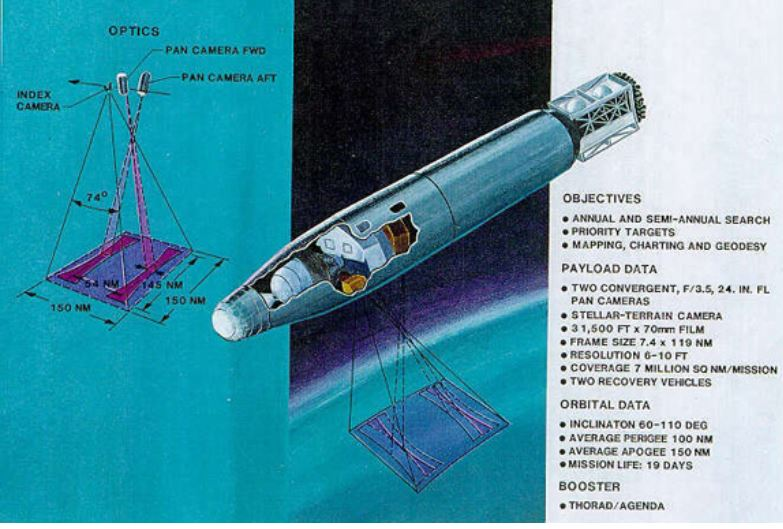
\includegraphics[width=.85\linewidth]{image/Electro-optical.JPG}
		\caption {A KH-4B CORONA satellite}
	\end{subfigure}%
	\begin{subfigure}{.5\textwidth}
		\centering
		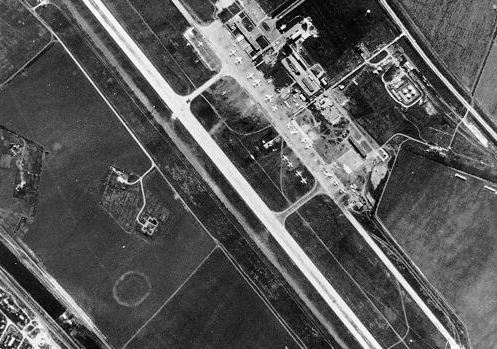
\includegraphics[width=.8\linewidth]{image/Fisrt corona photograph.JPG}
		\caption{CORONA-4 satellite image}
	\end{subfigure}
	\caption{A KH-4B CORONA satellite and imagery data taken over Soviet airfield \citep{ruffner1995corona}}
\end{figure*}
Additionally, we present data for each domain that show the chronological rise in the number of satellites carrying electro-optical sensor and imaging systems for various applications, identify technical and commercial in using existing EO for each application, and discuss the global market growth in EO payload system suppliers. However, the review does not include: (i) failed missions (i.e., a spacecraft equipped with an electro-optical imaging payload that was launched into space but failed during the launch, operation, or was unable to complete the intended mission), (ii) small spacecraft masses less than 1kg and greater than 500kg (i.e., 1 $<$ S/C mass $>$ 500 kg), and (iii) active imaging systems such as SAR, LIDAR, and others. 
\section{Early developments: 1960 - 1990}
During these decades, most of the development work was focused on experimenting with optical imaging and sensors such as panchromatic, TV cameras, scanners, various telescopes, and other imaging systems and sensors. In 1959, the United States launched the first successful reconnaissance satellite, CORONA \citep{ruffner1995corona}, which could capture images of the Earth's surface and had a single optical camera, but later in the program, three optical cameras were used, and many different types of optical cameras, such as J-3 and rotator cameras, were used. 
Around the 1960s and 1970s, satellite-based optical imaging system began to be used for collecting data for scientific research and monitoring natural resources, weather patterns, and other environmental variables; however, these systems were limited in their capabilities and were primarily used for military and intelligence gathering purposes. Specifically, the first Landsat satellite, equipped with a multispectral scanner optical payload capable of capturing images of the Earth's surface in multiple spectral bands, launched in the 1970s, ushered a new era of electro-optical imaging improvement.\\
In recent years, advances in optics, electronics, and materials science have led to the development of more sophisticated and capable sensors, such as advanced multi-spectral, super-spectral, hyper-spectral, SAR, and LIDAR sensors, which not only have a higher spatial resolution but can also capable of capturing data in much more precisely defined bandwidths or frequency ranges \citep{madry2013electro}. The primary drivers of each of these technologies, and eventually qualification were government entities; either space agencies or various branches of the military organization. In fact, at the time the main geopolitical entities capable of developing and implementing electro-optical imaging technologies in conjunction with the spacecraft bus were the United States and the former Soviet Union. And the majority of the early missions were technology demonstrators with purely scientific or technical ambitions, such as Explorer 6's optical scanning device \citep{judge1962observations}, which was intended to test the feasibility of optical instruments for capturing low-resolution daylight cloud-cover photographs. \\
In addition to the aforementioned first-of-their-kind missions, the US and USSR conducted a number of experimental spacecraft missions and endeavors, such as CORONA, Luna, TIROS, Nimbus, Landsat, and others, in which a variety of electo-optical imaging systems were tested and different data was gathered. Initially, the US launched 144 CORONA satellites into orbit to photograph Russia and China, which they dubbed the KH-x satellite system \citep{ruffner1995corona}, whereas the USSR launched a number of Luna missions into space with early technology demonstration optical the payloads to photograph the far side of the moon and later lunar exploration missions. Fig. 2 depicts one of the CORONA satellites, KH-4B, and its mission objectives of acquiring photography data as well as data collected over Soviet airfields.\\
Then the US TIROS mission continued the effort, with the successful launch of TIROS-1 equipped with specially designed miniature television cameras, infrared detectors, and videotape recorders, paving the way for a new generation of meteorological spacecraft and laying the groundwork for the subsequent development of instruments designed specifically for earth observation \citep{Tatem2008FiftyYO}. The TIROS program (Television Infrared Observation satellite) was NASA's first experimental step to determine if satellites could be useful in the study of Earth \citep{neeck2005nasa}. The 122 kg spin stabilized spacecraft included large and low resolution television cameras, and later the spacecraft had upgraded sensors \citep{neeck2005nasa}, had lifetimes of more than 3 years, and was used for routine and severe weather forecasting. The NOAA series of spacecraft succeeded the TIROS spacecraft and carried an instrument called the advanced very high-resolution radiometer, which measured resistance emanating from Earth in five spectral bands spanning the visible to infrared \citep{Tatem2008FiftyYO}. Although it was intended for meteorological purposes, this sensor was ultimately most successful for land and sea observation, providing multitemporal measurements on a global scale.\\ 
The Nimbus series spacecraft, which began in 1964, was also a landmark series because it continued the development of space-based meteorological observations from low-earth orbit (LEO) with advanced vidicon cameras, infrared radiometers, and rapid data access via the automatic picture transmission (APT) system \citep{neeck2005nasa, Tatem2008FiftyYO}. Later satellites in the series used microwave radiometers, atmospheric sounders, ozone mappers, and ocean color scanners to extend observations of Earth to include sea-ice coverage, atmospheric temperature, atmospheric chemistry, the earth's radiation budget, and sea-surface temperature. Furthermore, visible cameras, infrared and microwave radiometers, spectrometers, ultraviolet backscatter sensors, and coastal zone color scanners were among the Nimbus instruments.\\
In the early 1970s, NASA launched the Landsat series of satellites with various types of sensors providing essential data for improving our understanding of the Earth's atmosphere, oceans, ice and snow, and land. These were the MSS and TM sensors carried by Landsat spacecraft \citep{wulder2019current}, the AVHRR sensor carried by the NOAA spacecraft series \citep{oesterheld1998relation}, Sensors carried by SPOT spacecraft \citep{Tatem2008FiftyYO}, more recently NASA's ASTER sensors and the hype-spectral sensors \citep{prentice2021design} now used on many small satellite platforms for various purposes. \\
A key development from 1960 to 1990 was the use of multispectral sensors \citep{Tatem2008FiftyYO}, stimulated in part by the declassification of military satellites that used infrared and microwave to observe the Earth's surface.During the last decade of early optical sensor development, NASA has placed a renewed emphasis on small satellites, reflecting advances in compact sensor, small satellite bus, and launch vehicle technology, as well as management advancements.\\
Overall, the use of electro-optical imaging and sensors has been a significant advancement over the last three decades, and the technology has made significant technical and commercial progress. Furthermore, EO sensor technology has advanced at an unprecedented pace over the years, beginning in 1972 with the first multispectral satellite, Landsat-1, which had four spectral bands, to 1997 with the first hyperspectral satellite, Lewis, which had 384 spectral bands \citep{zhu2018review}. The spatial resolution has also improved considerably over the decades, from 80m in Landsat-1 to 31 cm in Worldview-3.  The electro-optical sensor technology has also proven the ability to perform a variety of functions and is increasingly being used in almost all spacecraft platform, from small satellites, including nanosatellites and micro-satellites, to larger earth observation satellites, to remote deep space missions \citep{chauhan2015hyperspectral}. 
\section{Sun-synchronous spacecraft}
Over the past five decades, technological advancements and the launch of sun-synchronous earth observation satellites have resulted in a huge growth in both revenue and the number of spacecraft carrying optical imaging sensor payloads and other instruments.  \\
The growing demand for high-quality remote sensing imagery data, combined with advances in optics, mechanics, and materials, as well as signal and data processing technology, are the primary drivers of the evolution of EO payload sensors, and have served as an impetus for the maturation of space-proven 0.5 m resolution or less \citep{demirel2005one, sandau2010status} electro-optical imaging system. These systems are critical components of spacecraft, providing imaging and sensing capabilities for a variety of uses including as earth observation, scientific research, defense, and other commercial applications. Furthermore, advancements in sensor technology, image data storage, processing, interpretation, analysis, and transmission have resulted in a paradigm shift in our ability to detect, analyze, and utilise imagery data from remote satellite platforms over the last decade \cite{arthur1997}. Table 1 presents all electro-optical imaging sensor-based small spacecraft launched from 1990 to the present.\\
The vast majority of Sun-Synchronous Orbit spacecraft carrying electro-optical imaging systems solely for the purpose of acquiring imagery data of the Earth for various applications.\\
The earliest successful operational use of an electro-optical system on an SSO small satellite was on the TUBSAT spacecraft, which was equipped with high resolution and hyper-spectral optical imagers \citep{roemer2003flight} for providing snapshot imaging capability of medium or high resolution ground scenes in disaster-affected areas. \\
However, since the introduction of small spacecraft, notably CubeSats in 1997, and as electro-optical technology has matured and SSO/LEO imaging mission requirements have increased, the use of electro-optical imaging system on SSO satellites has been revisited.
Parallel to the introduction of downsizing spacecraft, the fundamental limitation imposed by the electro-optical imaging system on the SSO spacecraft is its limited size, weight, and power (SWaP), as explained in section 5.  \\
Small satellites are designed to operate on significantly fewer budgets and resources than larger spacecraft, limiting the capabilities and performance of optical imaging payloads that can be carried onboard. Furthermore, since these smaller SSO platforms can only generate hundreds of watts due to the sun arising from the longer fraction of each orbit spent in Earth's shadow, they can typically only accommodate low power optical imaging equipment estimated at a few hundred watts \citep{selva2012survey}. \\
Despite the prevailing constraint of small spacecraft missions equipped with electro-optical sensors in various orbital regimes, numerous aspects change today's picture and potentially increase the use of electro-optical systems on SSO/LEO satellites and beyond:
\begin{enumerate}
	\item \textbf{Growing demand of earth observation imagery data}: There is an increasing demand for Earth observation data for a variety of applications, including environmental monitoring, disaster response, urban planning, and national security. In order to address this requirement, electro-optical remote sensing devices can deliver high-resolution, real-time data. Recent developments, such as the convergence of defense needs with commercial capabilities, call this paradigm into question. Furthermore, three types of stakeholders are involved  \citep{denis2017towards}: established commercial operators, so-called new space players wanting to turn space into a commodity, and states with new space ambitions as a tool of sovereignty and soft power.
	\item \textbf{Technology advancements}: Rapid advances in imaging sensor technology, image processing algorithms, and data transmission capabilities have significantly enhanced the performance and capacities of electro-optical systems. This has enabled the development of smaller, lighter, and more capable systems, which are well-suited for usage on small satellites.
	\item \textbf{Emergence of new mission and application}: The growing availability of spaceborne electro-optical imaging systems is allowing for the development of new applications and markets, including as precision agriculture, forestry management, marine surveillance, and air quality monitoring. Specifically, in the last four years, there has been a rapidly increasing commercial industry for employing the SSO earth observation satellite constellation \citep{sandau2010status} to provide high-quality imagery data access and coverage to broad regions of the world for monitoring and studying the Earth's environment.
	\item \textbf{Decreasing cost of space launch }: The cost of launching satellites into space has decreased considerably in recent years, making it more economical for a broader range of organizations and individuals to launch their own spacecraft along the various optical sensor, including CubeSats and SmallSats, for a variety of applications.
	\item \textbf{Standardization and miniaturization of CubeSats}: The standardization and dwindling of CubeSats and SmallSats has made it easier and more cost-effective to design, develop, and launch spaceborne electro-optical imaging systems that can offer high-resolution images and data for a fraction of the cost of typical bigger satellites.
	\item \textbf{Advancement of data processing and analytic}: The improvement of data processing and analytics is changing the way electro-optical data is utilized, allowing for more efficient and effective use of spaceborne electro-optical systems. It enables the extraction of important insights, enhances decision-making processes, and raises the overall usability of Earth observation data for a variety of applications, with the disruptive factor being that analysts and end-users increasingly rely on Web-based workflows \citep{sudmanns2020big}.  Furthermore, the onboard increased data storage capacity, real-time capabilities, enhanced image quality and information extraction, automation and machine learning, integration with other data sources, data fusion and multi-sensor integration contribute to this.
\end{enumerate}
\begin{table*}
	\small
	\caption {A spacecraft with an EO payload launched between 1990 and 2023} % title of Table
	\centering % used for centering table
	\scalebox{0.73}{
		\begin{tabular}{c c c c c c c c c c c c c c c c} % centered columns (4 columns)
			\hline\hline %inserts double horizontal lines
			S/C & Country & Launch & Mass [kg] & Instrut. & $f\#$ & GSD [m] & Spectral [$\mu$m] & FOV [deg] & Power [W] & Sensor & Ref.\\ [0.5ex] % inserts 
			Name & & Year & & type &  & range & range & & &type & &\\
			\hline % inserts single horizontal line
			UoSat-5 & UK & 1991 & 48.4 & Color CCD imager & f/24 & 350 & 0.61 $\sim$ 0.690 & N/A & 3.6 & CCD sensor & \citep{fouquet1992uosat}\\
			KITSAT-1 & S/Korea & 1992 & 48.6 & Color CCD imagers & f/5.7 & 200 & N/A & 60 & 30 & CCD sensor & \citep{kramer2008overview}\\
			PoSAT-1 & Postugal & 1993 & 50 & CCD imagers & N/A & 200 & N/A & N/A & 18 & CCD  sensor & \citep{kramer2008overview} \\
			KITSAT-2 & S/Korea & 1993 & 50 & CCD earth imagers & f/1.8 & 200 & N/A & N/A & 30 &  CCD sensor & \citep{kramer2008overview}\\	
			TUBSAT-B & German & 1994 & 45 & Hyper-spectral imagers & f/5.6 & 23 $\times$ 30 & 0.4 $\sim$ 1.1 & 0.35 $\times$ 0.5 & 3  & CCD array & \citep{eo2012}\\
			FASat-B & Chile & 1995 & 55 & CCD imagers & f/1.1 & 200 & 0.61 $\sim$ 0.90 & 6.5 $\times$ 4.8 & 25 & EEV CCD04-06 & \citep{kramer2008overview}\\		 
			OrbView-2 & USA & 1997 & 390 & Multi-spectral imager & f/2 & 1000 & 0.402 $\sim$ 0.885 & 1.5 & 165 &  N/A & \citep{eoportal}\\ 
			TechSat & Israel & 1998 & 48 & PAN imager & N/A & 52 $\times$ 60 & 0.5 $\sim$ 0.8 &  3 $\times$ 12 & 4.5 &  PULNiX CCD TM-720 & \citep{eoportal}\\
		    SEDSat-1 & USA & 1998 & 36 & PAN imager & f/1.8 & 100 $\sim$ 140 & 0.44 $\sim$ 0.95 &  10 & 16 & CCD array & \citep{bankston1994seds}\\
		    TMSAT-1 & Thailand & 1998 & 50 & Multi-spectral imager & N/A & 100 & N/A & 35 & N/A & 2D CCD array & \citep{ SWEETING1997423}\\
		    SAC-C & AUDBIF & 1998 & 472 & Multi-spectral imagers & f/3.1 & 175 & 0.48 $\sim$ 0.9 & 29.42 & 221 & CCD array & \citep{eoportal}\\
		    SUNSAT & S/Africa & 1999 & 64 & Multi-spectral imager  & N/A & 15 & 0.52 $\sim$ 0.87  & 3.715 & 30 & CCD array & \citep{kramer2008overview}\\
		    UoSAT-12 & Singapore & 1999 & 325 & PAN, MSS imager & f/3.4 & 10/36 & 0.45 $\sim$ 0.9 &  N/A & 20 &  2D CCD silicon & \citep{ kramer2008overview}\\
		    DLR-TUBSAT & German & 1999 & 45 & PAN TV imager & f/16 & 375 & 0.51 $\sim$ 0.85 & 6.9 $\times$ 5.336 & 10 &  Sony CCD array & \citep{eoportal}\\
		    KITSAT-3 & S/Korea & 1999 & 110 & Multi-spectral imagers & f/5.7 & 13.5 & 0.51 $\sim$ 0.9 &  3.8 & 15 & TC104 CCD & \citep{kim1999development}\\
		    TiungSat-1 & Malaysia & 2000 & 56 & Multi-spectral imagers & f/0.75 & 70 & 0.51 $\sim$ 0.89 & N/A & 35  & 2D CCD array &  \citep{kramer2002observation}\\
		    Tsinghua-1 & China & 2000 & 50 & Multi-sepectral imager & f/1.5 & 50 & 0.5 $\sim$ 0.89 &  15 & 35  & Kodak KAI-1001 & \citep{kramer2002observation}\\
		    ASUSat-1 & USA & 2000 & 6 & Multi-spectral imager & N/A & 500 & 0.42 $\sim$ 0.8 & 18 & 10 &  2D CCD array & \citep{kramer2002observation}\\
		    EROS-A & Israel & 2000 & 260 & PAN imaging system & f/3.5 & 2 & 0.5 $\sim$ 0.9 &1.5 & 300 & CCD array & \citep{eoportal}\\		    
		    MAROC-TUBSAT & Morocco & 2001 & 47 & PAN TV camera & f/6 & 250 & 0.4 $\sim$ 0.8 &  N/A & 8.5 &  CCD matrix array & \citep{ kramer2002observation}\\
		    Badr-B & Pakistan & 2001 & 68.5 & PAN CCD imager & N/A & 250 & 0.4 $\sim$ 0.7 & N/A & 25 & CCD array & \citep{eoportal}\\
		    BIRD & German & 2001 & 94 & Thermal infrared imager & f/2 & 372 & 3.4 $\sim$ 9.3 & 19 & 90 & CdHgTe Arrays & \citep{sandau2010status}\\
		    AlSAT-1 & Algeria & 2002 & 88 & Multi-spectral imager & f/2.5 & 32 & 0.52 $\sim$ 0.9  & 26.6 & 20 & Kodak linear CCD & \citep{bekhti2008power, rachedi2004alsat}\\ 
		    Haiyang-1A & China & 2002 & 367 & TIR/MSS imagers & f/2.2 & 250 & 0.402 $\sim$ 12.5 &  36 & 30 &  CCD array & \citep{eoportal}\\	
		    NigeriaSat-1 & Nigeria & 2003 & 100  & Multispectral imager & f/4 & 32 & 0.48 $\sim$ 0.92 & N/A & N/A & KLI-10203 CCD & \citep{ikpaya2017pursuit}\\		
		    OrbView-3 & USA & 2003 & 300 & PAN/MSS imagers & f/4.5 & 4 & 0.45 $\sim$ 0.9 & 50 & N/A & CCD array & \citep{kramer2002observation}\\
		    BilSat-1 & Turkey & 2003 & 130 & PAN/MSS imager & N/A & 12.2 & 0.45 $\sim$ 0.9 &  4.4 $\times$ 4.3 & 10 &   KAI-4000 CCD & \citep{yuksel2005bilsat}\\
		    DMCSat-1 & UK & 2003 & 100 & MMulti-spectral imager &  f/2.5 & 32 & 0.52 $\sim$ 0.90 & 26.62 & 20 & Kodak linear CCD & \citep{eoportal}\\
		    Haiyang-1B & China & 2004 & 400 & TIR/MSS imager & N/A & 250 &  0.402 $\sim$ 12.5 & 36 & $\sim$ 30 & CCD array & \citep{eoportal}\\		
		    XI-V & Japan & 2005 & 1 & CMOS imager  & f/1.8 & 3500 & 0.4 $\sim$ 0.7 &  35 & 1.1 &  QVGA CMOS array & \citep{ FUNASE2007707}\\		     	
		    Sina-1 & Iran & 2005 & 160 & PAN/MSS imagers & f/2 & 50 $\sim$ 250 & 0.5 $\sim$ 0.89 &  40 &14.4 &  RL4000 CCD array & \cite{abolghasemi2012design}\\     
		    TopSat & UK & 2005 & 115 & PAN/MSS imagers & N/A & 2.5 $\sim$ 5 & 0.4 $\sim$ 0.7 &  1.4 & 30  & CCD array & \citep{price2002topsat}\\
		    Beijing-1 & China & 2005 & 166 & PAN/MSS imagers &   N/A & 4 & 0.4 $\sim$ 0.9 &  30 & 12 & e2v CCD21-40 & \citep{da2006small}\\ 
		    EROS-B & Israel & 2006 & 290 & PAN imaging system & F/5 & 0.7 & 0.45 $\sim$ 0.9 &  1.5 & 300 & CCD TD sensor & \citep{eoportal}\\		
		    LAPAN-TUBSAT & Indonesia & 2007 & 56 & Hyper-spectral imagers & f/11 & 5 & 0.4 $\sim$ 0.7 &  0.35 & 2.5 & DXC-990P CCD & \citep{hardhienata2007lapan} \\
		    Egypt-1 & Egypt & 2007 & 165 & PAN/MSS imagers & f/5 & 7.8 & 0.51 $\sim$ 1.70 & 4 & 35 &  CCD array & \citep{metwalli2012combining}\\
		    Compass-1 & German & 2008 & 1 & CMOS color camera & N/A & N/A & N/A & 53 & 2 &   CMOS arry & \citep{scholz2009flight}\\	
		    CanX-2 & Canada & 2008 & 3.5 & CMOS color imager & N/A & N/A & 1200 $\times$ 1024 & 30 & 4 & CMOS array & \citep{ rankin2005canx}\\		    	   
		    SwissCube & Switzerland & 2009 & 1 & CMOS color imager & N/A & 188 $\times$ 120 & 0.02 $\sim$ 0.767 & 18.8 $\times$ 29.4 & 0.251 &  MT9V032 CMOS & \citep{noca2009lessons}\\		
		    DubaiSAt-1 & UAE & 2009 & 190 & PAN/MSS imagers & N/A & 2.5 $\sim$ 5 & 0.42 $\sim$ 0.89 &  N/A &  52.3 & CCD array & \citep{al2009dubaisat}\\		
		    RazakSAT & Malaysia & 2009 & 190 & PAN/MSS imager & N/A & 2.5 $\sim$ 5 & 0.45 $\sim$ 0.89 & 1.675 & 63 & Linear CCD array & \citep{eoportal}\\	
		    ZASat-002 & S/Africa & 2009 & 60 & PAN/MSS imagers & f/1.2 & 6.5 & 0.44 $\sim$ 0.89 &  40 & 65 &  CCD matrix & \citep{burger2006south} \\
		    DMCSat-2 & UK & 2009 &  96 & Multi-spectral imager & f/5& 22 & 0.52 $\sim$ 0.9 & 26.6 & 26.5 & Kodak KLI14403 linear CCD  & \citep{eoportal}\\	
		    Deimos-1 & Spain & 2009 & 88 & Multi-spectral imager & f/5 & 22 & 0.52 $\sim$ 0.9 & 26.6 & 26.6 & Kodak KLI14403 linear CCD & \citep{eoportal}\\ 	    
		    PRISM & Japan & 2009 & 8.5 & Multi-spectral imager & f/1.8 & 250 $\sim$ 1000 & 0.35 $\sim$ 1.054 &  30.7 & N/A &   Teledyne HyViSI & \citep{mouroulis2014portable}\\		
		    Alsat-2A & Algeria & 2010 & 120 & PAN/MSS imagers & N/A & 1.5 $\sim$ 10 & 0.45 $\sim$ 0.89 &  30 & 50 &  CCD array & \cite{kameche2016flight}  \\	
		    StudSat-1 & India & 2010 & 1.3 & CMOS imager & f/4 & 95 & N/A &  5.56 & 75 & KAC-9618 CMOS & \citep{eoportal}\\		    	
		    SICH-2 & Ukraine & 2011 & 176 & PAN/MSS imagers & f/5 & 41.4 & 0.5 $\sim$ 1.7 & 35 & 25 &  CCD191 array & \citep{eoportal}\\
		    NigeriaSat-2 & Nigeria & 2011 & 270 & Multi-spectral imager & N/A & 32 & 0.45 $\sim$ 0.9 &  45 & N/A & linear CCD arrays (e2v) & \citep{eoportal}\\		
		    X-SAT & Sigapore & 2011 & 106 & Multi-spectral imager & N/A & 10 & 0.52 $\sim$ 0.89 &  4.2 & 25 &  CCD array & \citep{eoportal}\\		         
		    Jugnu  & India & 2011& 3 & NIR imager & f/3.5 & 197 & 0.75 $\sim$ 0.85 &  N/A & 3.8 &  CCD array & \citep{eoportal}\\		      
		    SSOT & Chile & 2011 & 117 & PAN/MSS imager & f/16 & 1.45 $\sim$ 5.8 & 0.45 $\sim$ 0.9 &  0.94 & 180 &CCD-TDI & \citep{eoportal}\\	
		    RASAT & Turkey & 2011 & 95 & PAN/MSS imagers & f/4.5 & 7.5 $\sim$ 15 & 0.42 $\sim$ 0.73 &  2.46 & 22 &  Linear CCD array &  \citep{teke2016satellite}\\	
		    NigeriaSat-X & Nigeria & 2011 & 87 & Multi-spectral imager &  f/5 & 22 & 0.52 $\sim$ 0.9 &  26.6 & 20 &   Kodak KLI14403 CCD & \citep{eoportal}\\	    
		    Kanopus-V1 & Russia & 2012 & 450 & PAN/MSS imagers & f/1.79 & 2.5 $\sim$ 12 & 0.52 $\sim$ 0.86 & N/A & 300 &CCD array & \citep{eoportal}\\	
		    StSat-3 & S/korea & 2013 & 150 & hyper-spectral imager & f/2 & $<$ 50 & 0.4 $\sim$ 1.05 & 35 & 5 & HgCdTe CCD & \citep{lee2007compact}\\	
		    DubaiSat-2 & UAE & 2013 & 300 & PAN/MSS imagers & f/5.7 & 1 $\sim$ 4 & 0.55 $\sim$ 0.89 & N/A & 300 &  CCD-TDI sensor & \citep{bushahab2014cal}\\
		    GomX-1 & Denmark & 2013 & 2.66 & CMOS color imager & f/2.2 & 35 & 0.4 $\sim$ 0.75 &  N/A &  1.3 & CMOS sensor & \citep{gomspace2023}\\		 
		    BEESAT-3 & German & 2013 & 1 & CMOS imager & f/2.8 & 695 & N/A &  N/A & 5 & CMOS-328 & \citep{eoportal}\\		    
		    VNREDSat-1 & Vietnam & 2013 & 130 & PAN/MSS imagers & f/16 & 2.5 $\sim$ 10 & 0.45 $\sim$ 0.89 &1.5 & 180 & CCD array & \citep{eoportal}\\	
		    PROBA-V & EU & 2013 & 138 & Multi-spectral imager & f/6 & 100 $\sim$ 200 & 0.415 $\sim$ 1.76 &  34 & 43.2 &  CCD array & \citep{eoportal}\\		    
		    MCubed-2 & USA & 2013 & 1 & CMOS color imager & f/9.6 & 200 & N/A & N/A & 1.2 &  CCD array & \citep{bekker2010cubesat}\\		   
		    ChubuSat-1 & Japan & 2014 & 50 & VIS/TIR imagers & N/A & 10 & 0.4 $\sim$ 13.5 &  4.6 & 85 &  CMOS sensor & \citep{ Narusawa2012DEVELOPMENTOC}\\		
		    Rising-2 & Japan & 2014 & 43 & CCD/CMOS imagers & N/A & 5 & 0.4 $\sim$ 1.05 &  29 & 28.4 &CMOS sensor & \citep{sakamoto2010development}\\		    
		    KazEOSat-2 & Kazakhstan & 2014 & 185 & PAN imager & f/4.3 & 1 & 0.44 $\sim$ 0.85 & 6.75 & 93 &  CCD array & \citep{kurczynski2016possibilities} \\		 
		    ASNARO-1 & Japan & 2014 & 495 & PAN/MSS imager & N/A & 0.5 $\sim$ 2 & 0.4 $\sim$ 1.1 & N/A & 14 &  CCD-TDI & \citep{eoportal}\\		
		    Deimos-2 & Spain & 2014 & 310 & PAN/MSS imagers & f/5.7 & 0.75 $\sim$ 4 & 0.45 $\sim$ 0.89 &  1.2 & 300 &  CCD-TDI sensor & \cite{ pirondini2014deimos}\\		
		    ALL-STAR & USA & 2014 & 4 & CMOS imager & f/5 & N/A & 0.4 $\sim$ 1 &  10 & 4.5 &  CMOS sensor & \citep{eoportal}\\		 
		    VELOX-1 & Singapore & 2014 & 4.3 & CMOS color imager & f/10.5 & 20 & N/A & N/A & 28.8 &  CMOS sensor & \citep{bui2015system}\\		  
		    GRIFEX & USA & 2015 & 4 & PAN imager & N/A & 850 & N/A &  N/A & 2 &  CMOS sensor & \citep{eoportal}   \\
		    TripleSat & UK & 2015 & 447 & PAN/MSS imager & N/A & 0.8 $\sim$ 4 & 0.44 $\sim$ 0.91 & 15 & 140 & linear CCD array &\citep{eoportal}\\		     
		    AlSat-1B & Algeria & 2016 & 103 & PAN/MSS imagers & N/A & 12 $\sim$ 24 & 0.523 $\sim$ 0.9 &  N/A & 48 &  CCD-sensor & \citep{serief2017estimate}\\		      
		    AlSat-2B & Algeria & 2016 & 115 & PAN/MSS imagers & f/3.2 & 2 & 0.45 $\sim$ 0.89 &  N/A & 50 & CCD array & \citep{wahballah2020survey}\\	
		    GHGSat-D & Canada & 2016 & 15 & MSS (VIS/IR) imager & f/5 & 24 & 1.63 $\sim$ 1.675 &  12 & 26 & Headwall sensor & \citep{jervis2021ghgsat}\\	
		    BIROS & German & 2016 & 130 & VNIR imager & f/3.8 & 42.4 & 0.46 $\sim$ 0.93 & 19.6 & 50 & CCD-line array & \citep{lorenz2015remote} \\
		    LAPAN-A3 & Indonesia & 2016 & 116 & Multi-spectral imager & N/A & 18 & 0.41 $\sim$ 0.99 & 13.4 & 37 &  CCD array & \citep{khamsah2019development}\\		    
		    PeruSat-1 & Peru & 2016 & 430 & PAN/MSS imagers & f/6.4 & 0.7 $\sim$ 2.5 & 0.45 $\sim$ 0.89 &  N/A & 90 &  CCD-TDI & \citep{wahballah2020survey}\\	
		    Diawata-1 & Philippine & 2016 & 50 & Multi-spectral imager & N/A & 3 & 0.42 $\sim$ 1.05 &  27.8 & 39 & CCD array & \citep{eoportal}\\	
		    Aalto-1 & Finland & 2017 & 4 & VIS imager & f/1.9 & 100 & 0.5 $\sim$ 0.9 &  30 $\times$ 19 & 4.8 &  CMOSIS CMV4000 & \citep{mughal2021aalto}\\		
		    ASTERIA & USA & 2017 & 12 & CMOS imager & f/1.4 & N/A & 0.5 $\sim$ 0.9 & 28.6 & 24 &  CCD array & \citep{eoportal}\\		    
 		   VENµS & Israel & 2017 & 268 & Super-spectral imager & f/7 & 5.3 & 0.42 $\sim$ 0.91 &  2.2 & 800 &  CCD-TDI & \citep{eoportal}\\	
		    OptSat-3000 & Israel & 2017 & 368 & PAN/MSS imagers & f/7 & 2.5 $\sim$ 10 & 0.4 $\sim$ 2.5 & N/A & N/A &  HgCdTe FPA & \citep{qian2015optical}\\ 		
 		   Kanopus-V3/4 & Russia & 2018 & 490 & PAN/MSS imagers & f/1.79 & 2.1 $\sim$ 10.5 & 0.46 $\sim$ 0.86 &  N/A & 300 &  CCD array & \citep{spacef2018}\\
 		   TOMASat $R^3$ & USA & 2018 & 5 & Multi-spectral imger & f/1.6 & 44 & 0.43 $\sim$ 0.89 &  N/A & N/A &  LUPA 1300-2 Si:CMOS & \citep{eoportal}\\ 
 		   HySIS & India & 2018 & 380 & Hyper-spectral imager & f/2 & 30 & 0.4 $\sim$ 0.95 &  14.5 & 750 &  CCD sensor & \citep{sita2019automatic} \\
 		   Diwata-2 & Philippine & 2018 & 56 & Multi-spectral imagers & N/A & 4.7 & 0.43 $\sim$ 1.02 &  17.33 & 38 & N/A & \citep{violan2021flight}\\ 
 		   VISION-1 & UK & 2018 & 440 & PAN/MSS imagers & f/15.9 & 0.9 $\sim$ 3.5 & 0.45 $\sim$ 0.91 & 1.1 & N/A &CCD array  &\citep{eoportal}\\ 
 		   Luojia-1 & China & 2018 & 20 & Multi-spectral imager & f/2.8 & 130 & 0.46 $\sim$ 0.98 &  32.3 &  N/A & CMOS sensor & \citep{jiang2018potentiality} \\
 		  	    	    	    	                      	       	    	    	    	        	           		    		      		       	    
		\hline
		\end{tabular}
	}
\label{table:nonlin} % is used to refer this table in the text
\end{table*}

\begin{table*}
	\ContinuedFloat
	\small
	\caption {A spacecraft with an EO payload launched between 1990 and 2023} % title of Table
	\centering % used for centering table
	\scalebox{0.73}{
		\begin{tabular}{c c c c c c c c c c c c c c c c} % centered columns (4 columns)
			\hline\hline %inserts double horizontal lines
			S/C & Country & Launch & Mass [kg] & Instrut. & $f\#$ & GSD [m] & Spectral [$\mu$m] & FOV [deg] & Power [W] & Sensor & Ref.\\ [0.5ex] % inserts 
			Name & & Year & & type &  & range & range & & &type & &\\
			\hline % inserts single horizontal line
 		   Eaglet-1 & Italy & 2018 & 5 & Panchromatic imager & f/3 & 5 & N/A &  N/A & 5 &  CCD sensor &\citep{saggesenanosatellite}\\ 
 		   ESEO & EU & 2018 & 45 & multi-spectral imager & f/1.85 & 25 & N/A &N/A & 3.6 & VGA CMOS snsor & \citep{sunter2016design}\\ 
 		   RWASAT-1 & Rwanda & 2019 & 3.2 & Multi-spectral imager & f/2 & 10 $\sim$ 20 & 0.457 $\sim$ 0.91 &  6.4 & 8 &  CMOS sensor & \citep{verspieren2020store}\\ 			
			EROS-C & Israel & 2019 & 400 & PAN/MSS imagers & N/A & 0.7 $\sim$ 2.8 & 0.45 $\sim$ 0.9 &   1.5 & N/A &  CCD/CMOS-TDI & \citep{jacobsen2004use}\\
			ETRSS-1 & Ethiopia & 2019 & 65 & PAN/MSS imagers & N/A & 15 & 0.45 $\sim$ 0.89 & 7.317& 18 &  E2v CCD sensor & \cite{gadisa2023etrss1}\\ 
			 AeroCube-15 & USA & 2019 & 6 & SWIR InGaAs imager & f/2.77 & 276 & 0.4 $\sim$ 0.8 & 21.7 $\sim$ 17.5 & N/A &  InGaAs/CMOS sensor & \citep{mauerhan2021radiometric}\\ 
			CIRIS & USA & 2019 & 6 & TIR radiometric imager & f/1.8 & 166 & 7.5 $\sim$ 12.7 & 12.2 $\times$ 9.2 & 15 & N/A & \citep{osterman2016ciris} \\ 
			PhiSat-1 & EU & 2020 & $\sim$ 12 & TIR/Hyperspectral VNIR & f/4.1 & 75 & 0.4 $\sim$ 1 & 31 $\times$ 16 & 12  &  CMOS sensor & \citep{esposito2019orbit}\\ 
			 NAPA-1 & Thailand & 2020 & 6.8 & Multi-spectral imager & f/5.8 & 40 & 0.465 $\sim$ 0.630 & N/A & 17.5 & CMOS sensor & \citep{brouwer2021earth}\\ 
			TRISAT & Slovenia & 2020 & 5 & Multi-spectral imager & f/3.7 & 100 & 1.1 $\sim$ 1.67 &  4.6 & 8 &  InGaAs sensor & \citep{gunter2023}\\ 
			CE-SAT-2B & Japan & 2020 & 35.5 & Multi-spectral imager & f/1.8 & 5.1 & 0.4 $\sim$ 0.7 &  N/A & 40 &  CMOS sensor &\citep{matsuzawa2021night}\\ 			
			NEMO-HD & Canada & 2020 & 72 & Multi-spectral imager & N/A & 2.8 $\sim$ 5.6 & 0.4 $\sim$ 0.96 &  N/A & 31 &CCD sensor & \citep{eoportal}\\ 
		   NAPA-2 &Thailand & 2021 & 7.6 & Multi-spectral imager & N/A & 5 & N/A &  2.2 & 25 &  CMOS sensor & \citep{brouwer2022multi}\\
		   DMSat-1 & UAE & 2021 & 15 & Multi-spectral imager & N/A & 40 & 0.48 $\sim$ 0.88 & 10 & N/A &   CCD array & \citep{dmsat2021}\\  
		   STEP Cube Lab-II & S/Korea & 2022 & 9.6 & Multispectral imager & N/A & 10 & 0.38 $\sim$ 0.94 &  N/A & 17.89 &  CCD sensor & \citep{bhattarai2021development}\\ 
		   NACHOS & USA & 2022 & & Hyperspectral imager & f/2.9 & N/A & 0.29 $\sim$ 0.5 & N/A & N/A &  e2v CCD47-20 & \citep{love2021nachos}\\ 
		   HYPSO-1 & Norway & 2022 & 6.8 & Hyperspectral imager & f/2.8 & 30 $\sim$ 100 & 0.4 $\sim$ 0.80 &  0.0564 $\times$ 7.88 & 11.65  & SONY IMX249 sensor & \citep{grotte2021ocean}\\ 
		   MATS & Swedin & 2022 & 50 & Multispectral imager & f/7.3 & 200 & 5000 &  5.67 $\times$ 0.91 & 40 &  E2V-CCD42-10 & \cite{hammar2019wide, eoportal} \\
		   NEMO-AM & Canada & 2023 & 16.1 &  Multi-spectral imager & f/2.8 & 200 & 0.4 $\sim$ 1 &  4.46 & 30 &  Kodak CCD & \citep{eoportal}\\
		   EOS-SAT 1 & S/Africa & 2023 & 176.6 & PAN/MSS imagers & N/A & 1.4 $\sim$ 2.8 & N/A & N/A & 45 &  CMOS sensor & \citep{dragonfly2023}\\   	    	    	    	    	                      	       	    	    	    	        	           		    		      		       	    
\hline
\end{tabular}
}
\label{table:nonlin} % is used to refer this table in the text
\end{table*}
In addition to capturing and collecting images of Earth and other planetary bodies, electro-optical imaging systems have been widely used in a variety of fields due to their ability to capture and analyze electromagnetic radiation in the optical spectrum due to their broad range of coverage EM, high spatial resolution multi-spectral and hyperspectral capabilities, non-intrusive data collection, cost effectiveness, and scalability.
\begin{figure*}
	\centering
	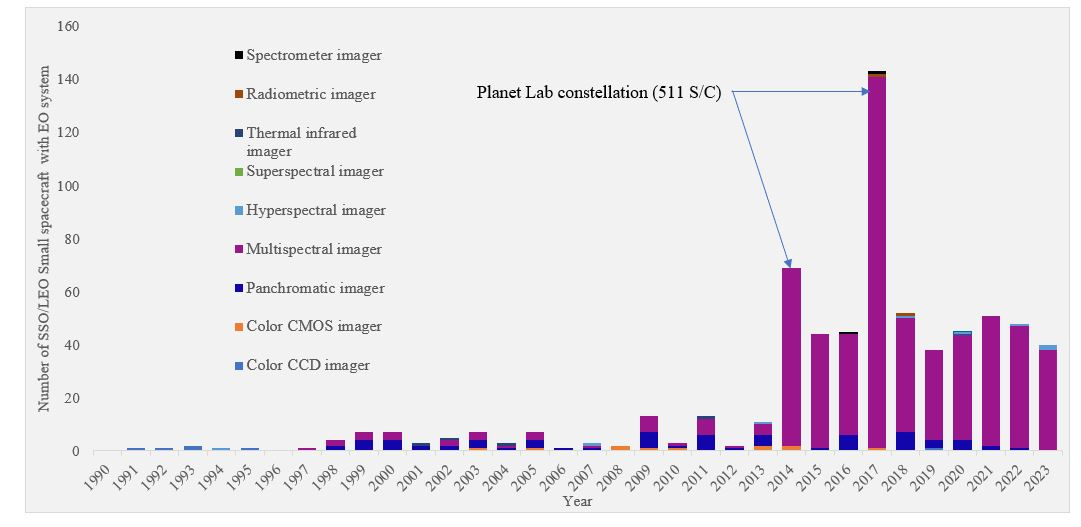
\includegraphics[width=1\linewidth]{image/No of SSO sat1}
	\caption{Number of SSo small satellites incorporating electro-optical imaging system by year and by optical imaging sensor subclass.}
	%\label{fig:my_label}
\end{figure*}
\subsection{small spacecraft constellation}
Small spacecrafts can present an opportunity for a cost-effective constellation to attain worldwide coverage on Earth with high time resolution, rapid replacement of a satellite, and soft degradation of system performance caused by the malfunction of one satellite \citep{sandau2010small}. Furthermore, a constellation of small satellite missions can provide comparable or greater mission capability than a monolithic satellite, but with significantly improved flexibility (adaptability, scalability, evolvability, and maintainability) and robustness (reliability, survivability, and fault tolerance) \citep{bandyopadhyay2016review}. \\
Specifically, data collected by optical imaging of an earth observation satellite constellation  could play a critical role in developing a scientific understanding of the earth system and its response to natural and human-induced changes, allowing for better prediction of climate, weather, and natural hazards for current and future generations. This has been demonstrated by NASA's recently launched 3U CubeSat TROPICS mission (Fig. 4a), a NASA constellation of six small satellites that will measure temperature, moisture profiles, and precipitation in tropical systems with unprecedented temporal frequency using microwave radiometer imaging sensors \citep{blackwell2018overview}.\\
However, number of small spacecraft constellation missions equipped with optical imaging systems have been launched, including the early constellation mission, DMC, and the current 36 Flock-4y of Planet Labs CubeSat constellation for optical observation with 3-5m resolution. \\
The DMC constellation began with the launch of AlSat in 2002, which is an advanced low-cost small spacecraft designed to monitor natural and man-made disasters and share imagery data with the constellation \cite{surry2002}. This spacecraft constellation consists of 5 small satellites equipped with optical imaging sensors that are networked together with the aim of delivering daily global imaging capabilities at medium resolution of 30-40 meters in 3-4 spectral bands for rapid response disaster monitoring and mitigation.  Later, in 2009, the second series of enhanced DMC satellites launched, providing vastly expanded imaging capacity, retaining the same 650 km swath width but with twice the pixel density at 22 meter GSD with significant enhancement and improvement of MTF and SNR \citep{surry2002}.  Subsequently, in 2018, a small spacecraft having a very high resolution capable optical imaging sensor with 2.5 m GSD panchromatic and 5 meter GSD multi-spectral capabilities was launched.\\
Planet Lab has flown over thirty successful CubeSat missions and deployed over 500 satellite constellation featuring optical imaging sensors, a telescope, and CCD cameras \citep{gutierrez2021automated} with a resolution of 3-5 meters in various batches for taking imagery across the Earth's Landmass.   It has three distinct small satellite constellations equipped with optical imaging sensor: Doves, SkySats, and RapidEye \citep{planet2023}. Dove (Flock) are roughly the size of a shoebox and weigh around 5 kg (Fig. 4b), which is many orders of magnitude smaller than conventional satellites, and they are often launched into space in large batches, known as "flocks."  The RapidEye, a commercial multi-spectral earth observation mission consisting of 5 mini-satellites weighing around 150 kg \citep{sandau2010small}, was launched into space in 2008, seven years before the Dove flock. Their objectives are to provide a variety of earth-observation products and services to a global user community with an optical imaging sensor capable of capturing five optical bands in the $0.4 \sim 0.85 \mu$m range and 6.5 m per pixel geometrical resolution at nadir \citep{sandau2010small}. The swath width is 80 km, with a maximum scene length of 1500 km per orbit. The RapidEye satellites amassed one of the largest archives of 5m resolution ever assembled and retired in 2020 \citep{planet2023}. Fig. 3 illustrates the number of small spacecraft equipped with electro-optical imaging systems by year and optical sensor technology subclass.\\
  \begin{figure*}
	\centering
	\begin{subfigure}{.5\textwidth}
		\centering
		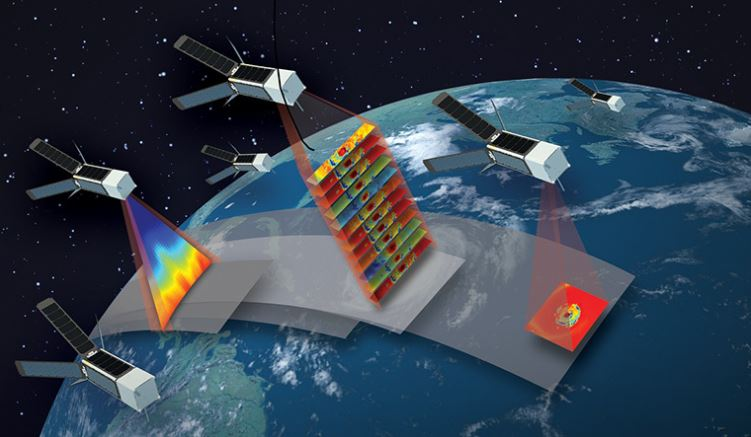
\includegraphics[width=0.85\linewidth]{image/Constellation of CubeSat.JPG}
		\caption{TROPICS, a constellation of 12 CubeSats flying in formation (Credit: MIT Lincoln Lab.)}
	\end{subfigure}%
	\begin{subfigure}{.5\textwidth}
		\centering
		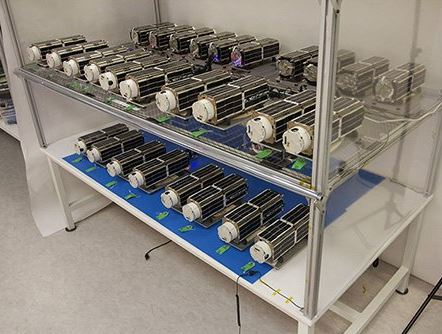
\includegraphics[width=.65\linewidth]{image/Planet Lab CubeSat constellation.JPG}
		\caption{Planet Labs CubeSat constellation (credit: Planet lab)}
	\end{subfigure}
	\caption{CubeSat constellation mission delivering imagery data to examine natural and human-caused changes to our planet Earth.}
\end{figure*} 
 Overall, a number of small spacecraft constellations equipped with optical imaging sensors have been launched and are in operation around the world, including Jilin-1, BlackSky, CORVUS, Zhuhai-1, Aleph-1, GHOSt-1, and others, with more anticipated to be launched in the future. 
\section{Deep space exploration spacecraft}
Over the course of a few decades, electro-optical-based spacecraft have been deployed in various orbital regimes, predominantly in LEO, but this is set to change as multiple nanosatellite missions are being launched beyond LEO now and in the near future. The recent MarCO CubeSat mission \citep{schoolcraft2017marco}, for example, which was equipped with two cameras with two lenses (NFOV and WFOV), has revolutionized the purpose of electro-optical payload systems beyond low earth orbit, legitimizing deep space and planetary exploration.   Furthermore, the new challenging scientific ambitions, combined with the variety and complexity of instruments, are increasingly detecting the system and mission design of space missions in general, and of deep space exploration missions in particular. \\
An electro-optical system is an appealing option for deep space exploration because it captures high-resolution images in various electromagnetic spectral bands, allowing for detailed mapping and analysis and providing information about its composition, as well as its non-intrusiveness and real-time data transmission. However, because this potential is just now being realized as the capability of small spacecraft has increased, the analysis described in this section is based on fewer flight missions and is limited to the analysis presented above.\\
The detector that created the image in early deep space missions was vidicon, a vacuum tube resembling a small CRT (cathode ray tube) \citep{nas2023}. However, modern electro-optical payloads such as CCD and CMOS cameras are commonly used in deep-space spacecraft because they provide a way to capture and transmit visual data from distant objects in space. Additionally, planetary geology, in-situ exploration, cartography, 3D and spectral imaging, as well as navigation, are all strongly linked with the use of imaging systems based on CCDs and contemporary scientific CMOS (sCMOS) optical sensors \citep{Behnke2015IMAGINGSF}.
\begin{table*}
	\small
	\caption{Small spacecraft equipped with EO instruments for deep space exploration thru 2023} % title of Table
	\centering % used for centering table
	\scalebox{0.65}{
		\begin{tabular}{c c c c c c c c c c c c c c} % centered columns (4 columns)
			\hline\hline %inserts double horizontal lines
			S/C Name & Country & Launch & Mass [kg] & Instrument type & Mission Objective &  Spectral band[$\mu$m] & Sensor type & FOV[deg] & Power [W]  & Manufact. & Ref.\\ [0.5ex] % inserts 
			%Name & & Year & & &  & & & \\
			\hline % inserts single horizontal line
			%\textbf{Mini-satellite: 100 - 180 kg \cite{nasa}}\\
			Luna-3 & USSR & 1959 & 278.5 & TV imaging system & Photograph $\&$ return images of lunar far side  & N/A & N/A & 60 & 60 & OKB-1 & \citep{david2023, siddiqi2018beyond}\\
			Ranger-7 & USA & 1964 & 365.6 & Tv imaging system & Acquire close-up pictures of lunar surface & N/A &  vidicon & 25 & 200  & JPL & \citep{siddiqi2018beyond, mesner1965tv}\\
			Mariner-IV & USA & 1964 & 260.8 & TV camera & Return close-up images of red planet & 200/pixels  & vidicon & 1.05 & 310 &  JPL & \citep{siddiqi2018beyond, allen1966mariner}\\ 
			Ranger-8 & USA & 1965 & 366.87 & TV imaging system & Obtain high resolution imagery   & N/A &  vidicon & N/A & 200 & JPL & \citep{siddiqi2018beyond, Henin2021ImagingOS}\\
			& & & & & of the lunar surface $\&$ verification & & & & & & &\\ 
			Ranger-9 & USA & 1965 & 367 & Tv imaging system & Transmit high resolution of  & N/A &  vidicon & N/A & 200  & JPL & \citep{siddiqi2018beyond, Henin2021ImagingOS}\\
			& & & & & lunar surface $\&$ verification & & & &  & & &\\  
			Lunar Orbiter-I & USA & 1966 & 386.9 & Imaging system & Photograph smooth areas of lunar  & N/A & N/A & LO & 375  &  Boeing & \citep{siddiqi2018beyond, Henin2021ImagingOS}\\
			Mariner-VI & USA & 1969 & 381 & Mars TV  & Study surface and atmosphere & 0.4$\sim$0.7 & N/A &11$\times$14 & 449 &  JPL & \citep{siddiqi2018beyond, Henin2021ImagingOS}\\
			& & & & camera & of red planet & & & & &  & &\\  
			Mariner-VII & USA & 1969 & 381 & Mars TV & Study surface and atmosphere  & 0.4$\sim$0.7 & N/A & 11$\times$14 & 380 & JPL & \citep{siddiqi2018beyond, Henin2021ImagingOS}\\
			& & & & camera & of red planet & & & & & & & \\
			Pioneer-10 & USA & 1972& 258 & Imaging photo & Study Jupiter's atmosphere of Io $\&$ solar  & 0.39$\sim$0.72 & N/A & 2.3 & 155 & TRW & \citep{siddiqi2018beyond, gehrels1974imaging}\\
			& & & & polarimeter & wind parameters $\&$ dust distribution & & & & & & &\\
			Pioneer-11 & USA & 1973 & 258.5 & Imaging photo & Study asteroid belt, env't around  & 0.255$\sim$0.955 & N/A & 1.8$\times$0.16 & 155 & 1TRW & \citep{siddiqi2018beyond, fimmel1977pioneer}\\
			& & & & polarimeter & Jupiter $\&$ Saturn, solar wind $\&$ cosmic rays & & & & & & & &\\
			Suisei & Japan & 1985 & 139 & CCD UV  & Take UV images of the hydrogen corona & N/A & CCD & 1.85$\times$1.96 & 100 &  ISAS & \citep{siddiqi2018beyond, Henin2021ImagingOS}\\
			& & & & imaging & before $\&$ after Comet Halley's descending & & & & & & &\\
			Clementine & USA & 1994 & 227 & LWIR/HIRES & Study surface of moon $\&$ near  & 0.4$\sim$2.8 & CCD & 0.3$\sim$10 & 360 &  NRL & \citep{siddiqi2018beyond, nozette1994clementine}\\
			& & & & UV/NIR camera & Earth asteroid geographos & & & & & & &\\
			Deep Space-1 & USA & 1998 & 373 & Miniature Integrated & Tech. dev't $\&$ validation  & 0.45 $\sim$ 0.9 & CCD & 0.69$\times$0.78 &2500 &  Spectrum & \citep{rodgers2007advanced, siddiqi2018beyond}\\
			& & & & Camera $\&$ Spectrometer &  for future missions & & & &  &  Astro&\\
			Stardust & USA & 1999 & 305.4 & NAVCAM & Determine position of Comet $\&$ obtain & 0.38 $\sim$ 1.1 & CCD & 3.5 & 330 & Lockheed & \citep{siddiqi2018beyond, sandford2006organics}\\
			& & & & & high resolution images of nucleus & & & & &  Martin &\\
			SMART-1 & EU & 2003 & 287 & Advanced Moon & Investigating the Moon and studying  & 0.75 $\sim$ 0.95 & CCD & 12$\times$32 & 462 $\sim$ 1190 & EU & \citep{racca2002smart, Henin2021ImagingOS}\\
			& & & & micro-Imager & chemical elements in the lunar surface & & &  & & & &\\
			Philae & EU & 2004 & 97.9 & Rosetta Lander & Study element, isotopic, molecular and &0.47 $\sim$ 0.87 & CCD & N/A & 32 & EU & \citep{bibring2007rosetta, boehnhardt2017philae}\\
			& & & & Imaging System & mineralogical composition of Comet &  & & & & & &\\
			New Horizons & USA & 2006 & 401 & LORRI & Map, characterize surface composition, & 0.35 $\sim$ 0.85 & CCD & 0.29 & 245 &  APL/SwRI& \citep{stern2015pluto, weaver2009overview}\\
			& & & & & geologies, $\&$ morphologies of Pluto & & & & & & &\\
			Grail & USA & 2011 & 132.6 & MoonKam & To study lunar features such as  & 0.68 $\sim$ 0.9 & N/A & 2.7/22 & $\sim$ 700  & Lockheed& \citep{zuber2013gravity, williams2014lunar}\\
			& & & & & craters, highlands, and maria  & & & & &  Martin&\\
			Yinghuo-1 & China & 2011 & 115 & optical imaging system & Capture high-quality images & N/A & CMOS & $\sim$ 360 & 90  & CNSA & \citep{zheng2013china, hua2008yinghuo}\\
			& & & & & of the Martian surface from orbit & & & & & & &\\
			DSCOVR & USA & 2015 & 440 & Polychromatic Imaging & Provide continuous solar wind measurements  & 0.4 $\sim$ 1.1 & CCD & 0.62 & 32   & Lockheed & \citep{eoportal, marshak2018earth}\\
			& & & & Camera (EPIC) & for accurate space weather forecasting& & &  & &  Martin &\\
			MarCO & USA & 2018 & 13.5 & Miniature Wide and & To relay and verify deployments and  & N/A & CMOS & 138/6.8 & $\sim$ 35 &  JPL & \citep{schoolcraft2017marco, jpl2018}\\
			& & & & Narrow field camera & capture outreach images during entry, & & & & & && &\\
			& & & & & decent $\&$ landing of InSight mars mission & & & & && & &\\
			CHEOPS & EU & 2019 & 273 & Optical space camera & To determine size of known extrasolar  & 0.4 $\sim$ 1.1 & CCD (E2V & 0.32 & 60 &  Airbus & \citep{broeg2013cheops, fortier2014cheops}\\
			& & & & & planets & & & CCD47-20) & & & & \\
			EQUULEUS & Japan & 2022 & 12 & PHOENIX/DELPHINUS  & Characterize radiation env't in geospace & 0.4 $\sim$ 0.8 & CCD & 11.9 & $\sim$50 &  JAXA & \citep{funase2020mission, ikari2019solar}\\
			& & & & imager & by imaging the Earth’s plasmasphere & & & & & &  &\\
			LunIR & USA & 2022 & 14 & MWIR optical camera & Capture and downlink MWIR images &  3 $\sim$ 5 & MWIR & 22.8 & $<$ 15 &   Lockheed & \citep{martinez2021advanced, crusan2019nasa}\\
			& & & & & of lunar surface & & & & &   Martin &\\
			NEA Scout & USA & 2022 & 14 & NEA Scout camera & Perform reconnaissance of an asteroid $\&$ & 0.4 $\sim$ 0.9 & CMOS & 27 & $<$ 5   & NASA & \citep{johnson2022near, mcnutt2014near}\\
			& & & & & to image the object at very high & & & & & & & \\
			& & & & & resolutions of up to 10 cm/pixel & & & & & & &&\\
			ArgoMoon & EU & 2022 & 14 & Optical camera & Take historical picture of desired target  & RGB & CMOS & 2.5/ 40 & 57.3 & 30   Argotec & \citep{di2019argomoon, molli2023design}\\
			& & & & & (ICPS, Moon and Earth), relay & & & & & & &\\
			& & & & &   mission data and test optical comm.  & & & & &  & &\\
			%\textbf{Micro-satellite: 10 - 100 kg \cite{nasa}} & & \\ [1ex]
			\hline
			% \textbf{Nanosatellite: 0.01 - 1 kg \cite{nasa}} & & \\ [1ex] % [1ex] adds vertical space
		\end{tabular}
		%\label{table:nonlin} % is used to refer this table in the text
	}
\end{table*}
At least 25 small spacecraft have been launched beyond LEO for deep space research since the first Sputnik 1, including the recent CubeSat, ArgoMoon on the Artemis 1 mission, each equipped with an electro-optical payload such as CCD and CMOS cameras and high-resolution instruments \citep{hambleton2016international}. A CCD is often a large-scale integrated circuit with a two-dimensional array comprising hundreds of thousands or millions of charged-isolated wells, each of which represents a pixel, while some CCD imagers have detectors consisting of single lines of CCD sensors \citep{nas2023}. \\
Depending on the mission requirements, SNR, and electrical power consumed by a deep space spacecraft's electro-optical payload ranged from several watts (Mariner-7) to a few 0.0573 kW \citep{di2019argomoon} (most demanding optical data communication mode on ArgoMoon). Table 3 show successful deep space spacecraft missions weighing less than 500 kg which employed electro-optical technology thru 2022. The low number of flights is primarily due to the high risk and expense involved with deep space missions; however, the table shows that, over time, confidence in electro-optical payload technologies has grown, resulting in an increasing number of deep space spacecraft using EO payload systems.\\
The United States, Japan, and the European Union are the current leaders in deep space missions that use an EO payload, and some African and Asian countries have lately become involved in the commercialization of the EO payload system. These nations are likely to launch a rising number of electro-optical payload-based small satellites for deep space exploration in the years to come, maintaining their leadership in this domain.\\
In addition to allowing spacecraft to acquire imagery data of the Earth and other celestial bodies, an electro-optical system provides the benefits of high-resolution photography, non-intrusive data transfer, and real-time data communication. This has proven particularly effective in the older Luna-3 mission \citep{siddiqi2018beyond} to the recent MarCO \citep{schoolcraft2017marco} and ArgoMoon CubeSat missions \citep{di2019argomoon}, for example, where they constitute a landmark and guidelines for future space exploration based on small spacecraft equipped with an electro-optical payload. \\The electro-optical payload on ArgoMoon, in particular, consists of two distinct optical cameras \citep{di2019argomoon} with narrow(2.5$^\circ$) and wide(40$^\circ$) field of view (FoV) weighing up to 1.2 kg, allowing for maximum performance in tracking and capturing highly detailed scientific photos of the most important locations (e.g., ICPS, CubeSats, Moon, and Earth). Furthermore, while the wide FoV camera is able to capture a bigger section of the sky to rapidly scan the space around the satellite looking for the target, the narrow FoV payload works like a telescope, being able to acquire detailed pictures of the target with different resolutions according to the distance\citep{simonetti2020argomoon}. Considering the ICPS dimensions of around 5 meters in diameter, the photos’ resolution is 1 px/cm from a distance of 100 meters, 1 px/dm from 1000 meters, and so on, reducing the distance \citep{simonetti2020argomoon}. Both payloads work in a correct spectrum due to the lens coating that filters out unwanted frequencies and are equipped with a high-speed CMOS image sensor with a resolution of 4096x3072 pixels \citep{simonetti2020argomoon}. Another instance of an electro-optical system providing a high degree of observation in deep space was on the Near-Earth Asteroid Scout), the NASA/MSFC/JPL 6U CubeSat that performs reconnaissance of an asteroid, taking pictures and observing its position in space using NEA Scout optical camera \citep{mission2022nea}. The monochromatic version of the CMV20000 CMOS detector used in the OCO-3 is integrated in the NEA Scout optical camera, which weighs 0.39 kg and has a 27$^\circ$ FOV, f/2.8, 50.2 mm, and IFOV=0.09mrad/pixel \citep{mission2022nea}. And Japan's EQUULEUS 6U CubeSat equipped with two optical instruments \citep{funase2020mission} (PHOENIX to conduct imaging of the Earth's plasmasphere using extreme ultraviolet wavelengths, and DELPHINUS to to observe impact flashes of meteoroids on the far side of the moon).\\
The advantages of an electro-optical-based deep space spacecraft mission for collecting high-resolution image data will continue to entice space organizations to use and develop new technologies. Several near-term missions, including INSPIRE (COTS payload processor with imager) \citep{klesh2013inspire, jpl2023}, Multi-angles imagers for aerosols (MAIA) (UV-VNIR-SWIR spectropolarimetric camera) \citep{liu2017multi, jpl2023}, Janus and Lunar Trailblazer (ECAM visible camera) \citep{shoer2021janus, arthur1997, jpl2023}, and another electro-optical payload small spacecraft, were proposed for deep space exploration mission. Most proposed missions require the incorporation of modern electro-optical sensors, cameras, and other equipment to the spacecraft in order to collect imagery and other telemetry data, and if successful, could enable a much greater utilization of an electro-optical camera and other instruments for deep space missions.
\begin{figure*}
	\centering
	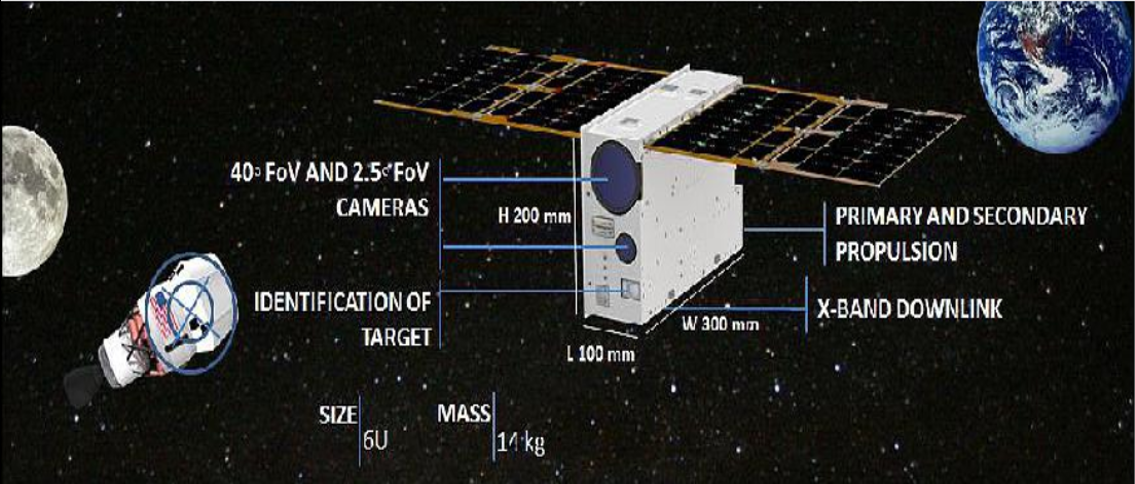
\includegraphics[width=.9\linewidth]{image/ArgoMoon satellite equipped optical payload.png}
	\caption{ArgoMoon CubeSat equipped optical camera and other payload \cite{di2019argomoon}}
	%\label{fig:my_label}
\end{figure*}
\section{EO-COTS of small spacecraft under 100 kg}
Small satellites, such as mini-satellites, micro-satellites, and nano-satellites, have become a rapidly expanding niche in the space industry in recent years due to their inexpensive cost and relatively simple design \citep{poghosyan2017cubesat}. Over 450 small satellites (those weighing less than 500 kg) went into orbit between 2012 and 2022, with an additional 18,500 anticipated to be deployed in the next decade (2022-2031) \citep{euro2022}.  These spacecraft have been outfitted with a variety of optical payload systems, such as cameras, spectrometers, and other sensors, which have opened up new possibilities for commercial applications such as earth observation, telecommunications, and scientific research in tandem with their payload system. Moreover, a nano-satellite mission, specifically a more advanced CubeSat mission, has recently been developed and proposed for scientific research and technology development, indicating that CubeSats have clearly begun to transition from being solely educational and technology demonstration platforms to offering opportunities for low-cost real science missions with significant value in terms of science return and commercial revenue \citep{poghosyan2017cubesat}.\\
In parallel to this commercial push, private, government, and various institutions have been conducting research and development into the use of COTS optics and sensor components. In particular, an experimental satellite built by universities, such as the UoSAT and TUBSAT series of spacecraft \citep{kramer2008overview}, has provided the foundation for realizing low-cost satellites with adequate EO payload for earth observation capabilities. \\
Today, a whole generation of universities and NewSpace companies have leveraged such cost-effective spacecraft development in the small satellite ecosystem and have taken advantage of the rise in computing capabilities to produce much greater progress in the last two decades. Furthermore, the growth of nanosatellites, including CubeSat, has increased interest in the COTS of EO instruments, as well as the translation of academic research interest into the development of innovative new-space EO ventures such as Planet Labs, which has flown over 200 satellite-equipped EO payloads for various applications \citep{curtis2023}.\\
It should be noted that, due to the nature of the small satellites industry, which is dominated by many small private enterprises or academic organizations, information on flight systems can be limited or non-existent. Subsequently, what is presented in this section contains less information on electro-optical system attributes such as resolution, FoV, SNR, data storage and transmission rate, and SWaP factor and more in-depth study on specific commercial EO technologies suited for small satellites and their space applications. Moreover, This section provides an overview of EO instrument commercialization, market trends, and the many EO technologies available in the global marketplace.Many COTS Small spacecraft EO payloads are available on the worldwide market, and Table 4 lists electro-optical cameras that are available on the global market. 
\subsection{EO-COTS market trends and commercialization}
One of the main factors driving the market trend toward small spacecraft optical payload systems is the growing demand for earth observation data, which is rapidly changing, as well as the various business models of companies operating across the value chain \citep{simer2023, cronje2023}. These data sets are all gathered by spacecraft platforms hosting the EO payload instruments, which are precision engineered to collect data in extremely harsh environments. This acquisition layer serves as the backbone for the earth observation industry and has a direct impact on the latest space/satellite/constellation service as-a-service business model \citep{simer2023,cronje2023}. As competition within this acquisition layer grows, specific market trends emerge that have a direct effect on the optical instruments chosen, as well as the platforms that support them. As new entrants into the earth observation payload market create new demand for sensor and processing technologies, EO payload designers, developers, and manufacturers must be aware of this shift in instrument demand and collaborate with service providers to address unique requirements such as optimizing instrument accuracy for specific applications and acceptable margin. Figure 4 depicts the electro-Optical payload system's cost-performance vs. precision optimization curve.
\begin{figure*}
	\centering
	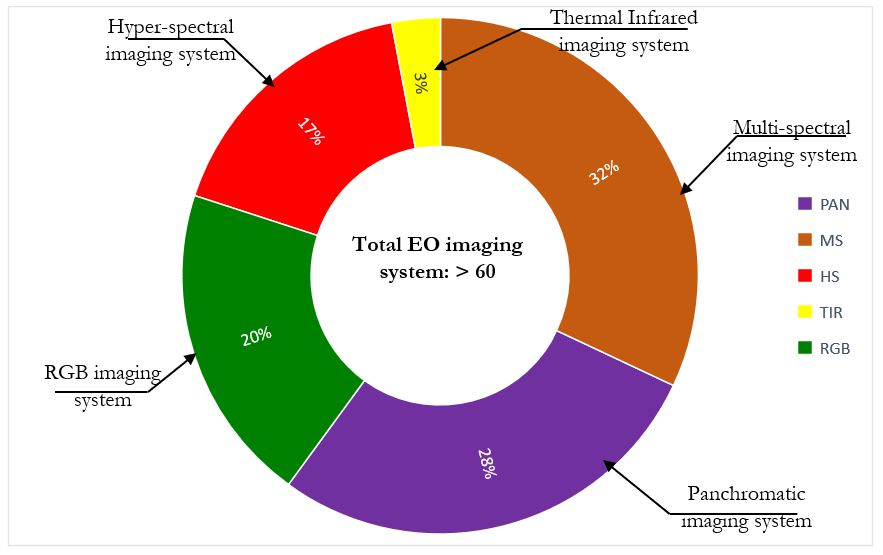
\includegraphics[width=.7\linewidth]{image/EO imaging system COTS.JPG}
	\caption{Percentage of electro-optical imaging systems for small satellites ($<$ 100 kg) accessible in the global market, divided by spectral bands.}
	%\label{fig:my_label}
\end{figure*}
\begin{table*}
	\small
	\caption{Small spacecraft electo-optical payloads available on the global market} % title of Table
	\centering % used for centering table
	\scalebox{0.76}{
		\begin{tabular}{c c c c c c c c c c c c c c c} % centered columns (4 columns)
			\hline\hline %inserts double horizontal lines
			EO-COTS  & Manufac. & Country & Mass [kg] & Spatial [m]  & Spectral & Power [W] & Target S/C & FOV [deg] & Sensor type & Reference\\ [0.5ex] % inserts 
			Name & & & & resoln.  & band type &  &  &  & \\
			\hline
			iSIM-90 (single & SATLANTIS & Spain & $<$ 4 & 1.65 & PAN, VNIR  &  25.3  &  12/16U & 15 & CMOS sensor &\citep{guzman2020compact, Satlantis2023}\\
			channel) & & & & & & (up to 4) & & & & & & & & \\
			iSIM-90 (dual  & SATLANTIS & Spain & $<$ 6 & 1.65 &  PAN, VNIR  &  30.5  &  12/16U & 15 & CMOS sensor &\citep{guzman2020compact, Satlantis2023}\\
			channel) & & & & & & (up to 8) & & & & & & & & \\
			iSIM-170 (single  & SATLANTIS & Spain & $<$ 8 & 0.8 & PAN, VNIR &  25.3  &  12/16U & 15 & CMOS sensor  &\citep{guzman2020compact, Satlantis2023}\\
			channel) & & & & & & (up to 5) & & & & & & & & \\
			iSIM-170 (dual  & SATLANTIS & Spain &  0.8 & 15 & PAN, VNIR & 30.5  & 12/16U & 15 & CMOS sensor &\citep{guzman2020compact, Satlantis2023}\\
			channel) & & & & & & (up to 5) & & & & & & & & \\
			GECKO & Dragonfly & South Africa & 0.4 & 39 & RGB (Bayer) & 2.6 & 1U/2U & N/A & N/A & \citep{casini2020towards, dragonfly2023}\\
			MANTIS-MS & Dragonfly & South Africa & 0.5 & PAN 16; &  6 $\times$ MS & 2.6 &  1U/2U & N/A & N/A & \citep{dragonfly2023}\\
			& & & & MS 32 &  & & & & & & & & & \\
			MANTIS-HS & Dragonfly & South Africa & 0.5 & 16 &  148 $\times$ HS & 2.6 & 1U/2U & N/A & N/A & \citep{dragonfly2023}\\
			CHAMELEON & Dragonfly & South Africa & 1.6 & PAN 10; & 7 $\times$ MS & $<$ 10 &  3U/6U & N/A & N/A & \citep{dragonfly2023} \\
			MS& & & & MS 32 &  & & & & & & & & & \\
			CHAMELEON & Dragonfly & South Africa & 1.6 & 20 $\sim$ 40 &  148 $\times$ MS & $<$ 10 &  3U/6U & N/A & N/A & \citep{dragonfly2023} \\
			HS& & & & to 20/40 &  & & & & & & & & & \\
			CAIMAN &  Dragonfly & South Africa & 1.8 & PAN 3; &  7 $\times$ MS & $<$ 10 &  6U & N/A & N/A & \citep{dragonfly2023} \\
			& & & & MS 6 &  & & & & & & & & & \\
			DragonEye & Dragonfly & South Africa & 18 & PAN 1.4; &  PAN +6 MS & 45 & 50 $\sim$ 100kg & N/A & N/A & \citep{dragonfly2023}\\
			& & & & MS 2.8 &  & & & & & & & & & \\
			RAPTOR & Dragonfly & South Africa & 45 & PAN 0.7; &  PAN + 6 MS & 45 &  50 $\sim$ 100kg & N/A & N/A & \citep{dragonfly2023} \\
			& & & & MSS 2.8 &  & & & & & & & & & \\
			TriScape-50 & Simera & South Africa & 0.37 & 29.3 & RGB & 7 & 1U & N/A & CMOS   sensor &\citep{casini2020towards, simer2023}\\
			MultiScape-50 & Simera & South Africa & 0.37 & 29.3 &  7 $\times$ VNIR & 7 & 1U $\sim$ 3U & N/A & CMOS sensor & \citep{casini2020towards, simer2023}\\
			HyperScape-50 & Simera & South Africa & 0.44 & 29.3 & 32 $\times$ VNIR & 7 &  1U $\sim$ 3U & 13.68 & CMOS sensor & \citep{casini2020towards, Simera2023}\\
			TriScape-100 & Simera & South Africa & 1.1 & 4.75 &  RGB with & 6 &  3U/6U & 1.66 $\sim$ 2.22 & CMOS  sensor & \citep{casini2020towards, Simera2023}\\
			& & & & &  NIR & & & & & & &  \\
			MultiScape-100 & Simera & South Africa & 1.1 & 4.75 & 7 $\times$ VNIR & 5.8 &  3U/6U & 2.22 & CMOS  sensor  & \citep{casini2020towards,  Simera2023}\\
			HyperScape-100 & Simera & South Africa & 1.1 & 4.75 &  32 $\times$ VNIR & 7 &  3U/6U & 2.22 & CMOS sensor & \citep{casini2020towards, Simera2023}\\
			TriScape-200 & Simera & South Africa & 12.1 & 1.5 & RGB with & 5.8 &12/16U & 1.2 $\sim$ 1.6 & CMOS sensor & \citep{Simera2023}\\
			& & & & &  NIR & & & & & & &  \\
			MultiScape-200 & Simera & South Africa & 12.1 & 1.5 & 7 $\times$ VNIR & 5.8 &  12/16U & 1.2 $\sim$ 1.6 & CMOS sensor  & \citep{Simera2023} \\
			IM200 & Clyde space & UK & 0.059 & N/A & Monochrome & 0.4 $\sim$ 1 & N/A & N/A & N/A & \citep{clyde2023}\\
			& & & & &  RGB & & & & & & &  \\
			XCAM C3D & XCAM & UK & 0.085 & 360 & RGB & 0.845 & 3U & 38 $\times$ 31 & CMOS sensor & \citep{casini2020towards, xcam2023}\\
			wHSI-100 & BST & Germany & 5.6 &  VNIR & N/A &N/A & N/A & N/A &  N/A &\citep{bst2023}\\
			HSI-100 & BST & Germany & 5.6 & 110 &SWIR & N/A & N/A & N/A & N/A & \citep{bst2023}\\
			HRVI-6HD & BST & Germany & 10.45 & 4.6 &  PAN/MSS & 25 &  N/A & N/A & N/A & \citep{bst2023}\\
			2ND GEN& & & & &  /HS & & & & & & &  \\
			HRVI-2HD & BST & Germany & 19 & 1.92 &  PAN + 4 $\times$ MSS & N/A  N/A & N/A & N/A & N/A &\citep{bst2023}\\
			SEEING & Safran & France & 6 & 1.5 &  MSS/HSS & 30 & 12U & 1.15$\times$0.76 & CMOS/CCD  sensor & \citep{safran2023}\\
			-1.5/0.75 & & & & & & & & & & & & &  \\
			SEEING-10 & Safran & France & 8 & 10 & MSS/HSS & 30 &  12U $\sim$ 18U & 6.3 $\times$ 4.3 & CMOS/CCD sensor & \citep{safran2023}\\
			SCS monitor & SCS space & South Africa & $<$ 3 & 6.5 & MSS & N/A &  12U & N/A & N/A & \citep{scs2023}\\
			nSight-2 & SCS space & South Africa & 6 & 16 &  MSS/HSS & 7 & 3U & N/A & N/A & \cite{scs2023}\\
			nSight-3 & SCS space & South Africa & 12 & 9.6 &  PAN/HSS & 10 &  6U & N/A & N/A & \citep{scs2023}\\
			TEGU & SCS space & South Africa &  PAN 2; & 24 & VIS-NIR & 35 &  50$\sim$100kg & N/A & N/A & \citep{scs2023}\\
			& & & MSS 4 & &  & & & & & & &  \\
			22mm camera & Kairospace & South Korea & $\sim$ 1 & 37 & RGB/NIR/PAN & 12 &  N/A & 12 & CMOS sensor  & \citep{kairo2023} \\
			22mm cluster & Kairospace & South Korea & 2.3 & 37 &  RGB/NIR/PAN & 48 &  N/A & 12 & CMOS sensor  & \citep{kairo2023} \\
			250mm camera & Kairospace & South Korea & $<$ 6 & 2.5 & PAN/MSS & 15 &  16U & 3 & CMOS  sensor & \citep{kairo2023} \\
			90mm camera & Kairospace & South Korea & 1.4 & Pan 3; & RGB/NIR/PAN & 4.2 &  6U & 1.5 & CMOS sensor & \citep{kairo2023} \\
			& & & & MSS 5 & &  & & & & & & & \\
			HyperScout-1 & Cosine RS & Netherlands & 1.5 & 47/67 &VNIR & 9  &  1U & 31$\times$16 & CMOS sensor & \citep{cosine2023}\\ 
			HyperScout-2 & Cosine RS & Netherlands & 1.8 & 47/67 & VNIR/TIR & 11 & 3U & 31$\times$16 & CMOS sensor  & \citep{cosine2023}\\ 
			HyperScout-M & Cosine RS & Netherlands & 1.2 & 39/55 & HSS/VNIR & 9 &  3U & 25$\times$12 & CMOS sensor  & \citep{cosine2023}\\ 
			HyperScout-S & Cosine RS & Netherlands & 1.6 & 19/28 &  HSS/VNIR & 9 &   3U & 13$\times$6 & CMOS sensor & \citep{cosine2023}\\ 
			Micro camera & Crystalspace & Estonia & $<$ 0.05 & $<$ 600 &  RGB & 0.75 & 3U & 44 $\times$ 34 & CMOS sensor  & \citep{slavinskis2015estcube}\\ 
			CGC001 & CG Satellite & China & $<$9.8 & PAN $<$ 1  & PAN & 85 &  50$\sim$100kg & N/A & CMOS sensor & \citep{cgsat2023} \\
			& & & & MSS $<$ 4 & &  & & & & & & & \\
			CGC002 & CG Satellite & China & $<$ 7 & 11.5 &  PAN/MSS/NIR & $<$ 15 &  3U & N/A & CMOS sensor  & \citep{cgsat2023}\\
			CGCV01 & CG Satellite & China &  24 & 1 & PAN & 25 &  50$\sim$100kg & N/A & CMOS sensor & \citep{cgsat2023} \\
			CGCMN01 & CG Satellite & China & $<$ 3 & $<$ 1.5 &  PAN/MSS & $<$ 13 & 3U & N/A & CMOS sensor & \citep{cgsat2023} \\
			CGCNL01 & CG Satellite & China & 5 & $<$ 50 & PAN & 9 & 6U & N/A & CMOS & \citep{cgsat2023} \\
			CGCMS01 & CG Satellite & China & $<$ 27 & PAN $<$ 5; &  PAN/MSS & 35 &  50$\sim$100kg & N/A & CMOS sensor & \citep{cgsat2023}\\
			& & & & MSS $<$ 20 & &  & & & & & & &  \\    
			ECAM-C50 & MSSS & USA & 0.59 & 2592 $\times$ 1944 & Monochrome & 1.6 &  N/A & 62 $\times$ 80 & CMOS  sensor & \citep{malin2023}\\
			ECAM-IR3S & MSSS & USA & 0.74 & 640 $\times$ 480 & LWIR & 2 &  N/A & 25 $\times$ 32 & CMOS sensor & \citep{malin2023}\\
			ECAM-P50 & MSSS & USA & 0.825 & 2592 $\times$ 2048 &  Monochrome & 3.25 & N/A & 90 $\times$ 109 & CMOS sensor  & \citep{malin2023}\\
			& & & & &   RGB Bayer & & & & & & & &\\
			ECAM-IR3A & MSSS & USA & 0.525 & 640 $\times$ 480 &  LWIR & 2 &  N/A &  36 $\times$ 48 & CMOS sensor  & \citep{malin2023}\\    
			LCAM & MSSS & USA & 0.88 & 2592 $\times$ 2048 &  Monochrome & 5.5 &  N/A &90 $\times$ 113 & CMOS sensor & \citep{malin2023}\\  
			DCAM & MSSS & USA & 2.4 & 2592 $\times$ 2048 & Monochrome & 15 &  N/A & 25$\times$32 & CMOS  sesnor & \citep{malin2023}\\  
			DISC & SDL & USA & 0.7 & 1024 $\times$ 1024 &  RGB/HSS & 1 &  N/A & N/A & N/A & \citep{sdl2023}\\
			SV-24 & L3Harris & USA & 10 & 0.9 $\sim$  1.1 &  visible PAN & 10 & 3U/6U & N/A & N/A & \citep{harris2023}\\
			SV-35 & L3Harris & USA & 20 $\sim$ 35 & 0.7 $\sim$ 1.1 &  PAN/MSS & 70 &  50 $\sim$ 100kg & N/A & N/A & \citep{harris2023}\\
			Monitor camera & Meisei & Japan & 1.1 & 1280 $\times$ 1024 & N/A & 4 & N/A & 30 $\times$ 24 & CMOS sensor &  \citep{meisei2023}\\ 
			piCAM & SkyFox & Czech Republic & 0.04 & 640 $\times$ 480&  RGB & 0.315 &  2U/3U & 76 $\sim$ 170 & CMOS sensor & \citep{skyfox2023}\\ 
			SCS & microgic & Israel & 0.56 & 10 &  N/A & 1.85 &  N/A & 75 $\times$ 64 & CMOS  sensor & \citep{micro2023}\\
			NanoCam  & GOMspace & Denmark & 0.277 & 2048 $\times$ 1536 &  RGB & 1.3 &  1U & N/A & CMOS sensor  & \citep{gomspace2023}\\
			\hline
			% \textbf{Nanosatellite: 0.01 - 1 kg \cite{nasa}} & & \\ [1ex] % [1ex] adds vertical space
		\end{tabular}
	}
	\label{table:nonlin} % is used to refer this table in the text
	\vspace{1ex}\\
	\raggedright{Note that: \textit{A "U" is a unit of measurement for CubeSats, representing one 10 cm $\times$ 10 cm $\times$ 10 cm cube. Thus, a "3U" satellite comprises of three 10 cm cubes yielding total spacecraft dimensions of 30 cm $\times$ 10 cm $\times$ 10 cm}}
	
\end{table*}
Another factor driving the commercialization of small spacecraft optical payload systems is the rapid pace of technological innovation, particularly in the miniaturization of components, material science, optics, microelectronics, and software which has resulted in the development of highly capable and sophisticated optical payloads that can be carried by small satellite platforms. These EO payloads can acquire high-resolution photos, collect spectroscopic data, and monitor a number of environmental factors with great accuracy and precision. Furthermore, it can be used for scientific research, space exploration, and telecommunications, in addition to earth observation and investigating the atmosphere, oceans, and other environmental factors, as well as observing weather patterns, climate change, and other global occurrences.\\
Overall, with ongoing technological innovation and increased demand for Earth observation data, and as companies and organizations seek to leverage the power of these small and flexible optical payloads for a wide range of commercial applications, the market trend and commercialization of small satellite optical payloads is expected to grow in the coming years. 
Despite the growing market trend toward small satellite optical payloads in the commercial market to perform new and demanding missions that require electro-optical systems, and the requirement to acquire imagery data from our planet and beyond, there are still a few hurdles to overcome. One of the most difficult challenges is developing standardized interfaces and protocols to ensure interoperability and compatibility among various subsystems, as well as improved reliability and durability to ensure that they can function in harsh space environments for extended periods of time. Furthermore, rising concerns about space debris as a result of increased satellite payload launches, combined with tight government rules related to spacecraft launches, are expected to hinder the expansion of the EO industry. Ultimately, the growing technological and commercial expansion of electro-optical systems  for small satellites must address the following requirements:
\begin{enumerate}
	\item \textbf{\textit{Low SWaP factor}}: The SWaP factor of an elctro-optical payload is one of the critical difficulties associated with small spacecraft since they have limited volume and must adhere to stringent size, weight, and power (SWaP) constraints without sacrificing system performance. Size and volume constraints are sometimes the most stringent payload limits, because payload performance is typically significantly dependent on its size and volume. An electro-optical payload system's aperture size, for example, determines its diffraction-limited angular resolution which in turn affects ground resolution \citep{selva2012survey}: 
	$$\Delta\chi \approx h*\Delta \theta = h*2.44 \frac{\lambda}{D}$$ where $\Delta\chi$ is the ground spatial resolution, $\Delta\theta$ is the diffraction limited angular resolution, $h$ is the orbit altitude, $\lambda$ is the wavelength, and $D$ is the instrument aperture size. volume constraint implies the design of electro-optical imaging payloads for small satellites must prioritize compactness, and low power consumption, which necessitates the employment of cutting-edge technology such as small sensors such as CCD and CMOS, low-power electronics, and lightweight materials. 
	\item \textbf{\textit{Resolution figure-of-merit (FoM)}}: Sensor technology and optics advancements led to in higher-resolution imaging capabilities of  electro-optical payloads which enable a more thorough and accurate remote sensing, mapping, and monitoring of the Earth's surface, as well as enhanced targeting and reconnaissance for defense applications. Subsequently, the small spacecraft electro-optical payload system is linked with the passive electro-optical subsystem to achieve the most possible ground sampling at the lowest possible cost, as well as the most promising potential for high resolution imaging \citep{shahin2021design}. Furthermore, each image resolution has a figure-of-merit that effects the image quality acquired by optical devices. MTF and GSD are real figures of merit for spatial resolution, whereas SNR, NEI, NE$\Delta \rho$, and NESR are figures of merit for radiometric resolution that help in the specific sensitivity requirements of optical equipment \citep{lomheim2002translation}. 
		\begin{figure*}
		\centering
		\begin{subfigure}{.5\textwidth}
			\centering
			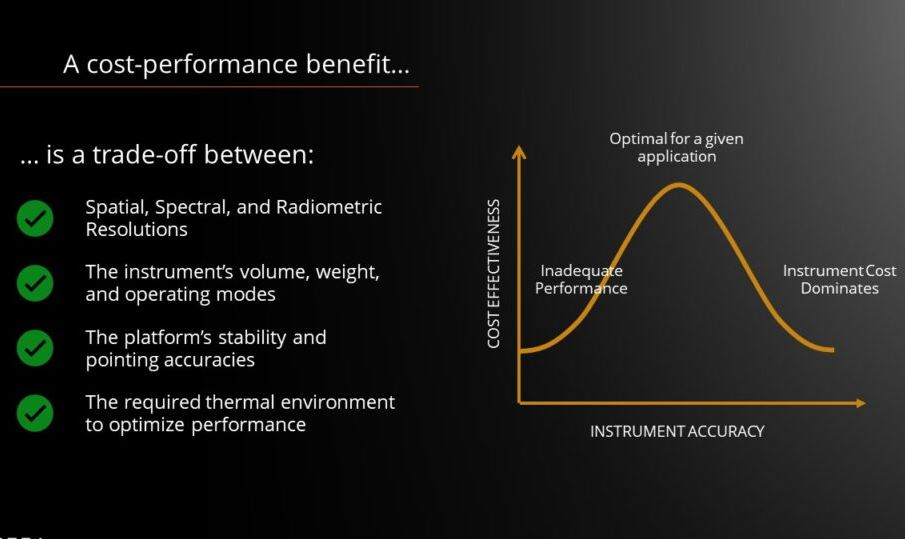
\includegraphics[width=.85\linewidth]{image/cost benefit of EO payload.JPG}
			\caption{Cost performance and optical imaging accuracy optimization curve \cite{simer2023}}
		\end{subfigure}%
		\begin{subfigure}{.4\textwidth}
			\centering
			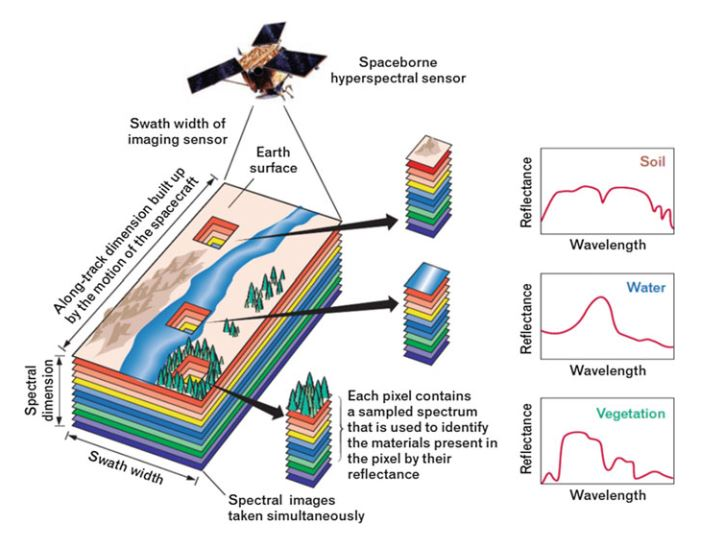
\includegraphics[width=.7\linewidth]{image/HSS sensor.JPG}
			\caption{Hyper-spectral imaging system \cite{sastry2020advances, shaw2003spectral}}
		\end{subfigure}
		\caption{EO optical imaging accuracy optimization curve and hyper-spectral imaging system}
	\end{figure*}
	\item \textbf{\textit{Change of modus of operandi}}: The business model shift and modus of operandi of electro-optical payloads have changed in recent years, becoming agile, cost effective, and collaborative, with an increased emphasis on sustainability and data as a service model \citep{sim2023}. The amount of data generated by electro-optical instruments is enormous, and as an element of autonomy, different data types of fusion, and transformation of raw data into intelligence is required, the entire data acquisition and mode of operation of optical instruments must be re-thought and re-designed to accommodate different requirements.  
	\item \textbf{\textit{Cost-performance optimization}}: Early on, optical instruments and platforms dominated whole missions where accuracy was the be-all and end-all. However, as piggybacking into orbit becomes more common because to its low cost, we are seeing a huge increase in the number of small spacecraft \citep{sim2023} adopting a fit-for-purpose approach. The low cost of CubeSats, in particular, limits the entire cost of an electro-optical system to no more than the overall cost of the spacecraft, and designers think of optimizing the instrument's precision for a specific application as well as tolerable error margin. Hence, finding the appropriate technique for reaching the optimal cost benefit versus optical instrument accuracy sweet spot while designing and manufacturing an optical payload without sacrificing performance is critical, as depicted in Fig. 7
	\item \textbf{\textit{High-data throughput}}: As the current earth observation industry and demand for high quality imaging data grows, spatial and spectral resolution rise, meaning more data and pixels are processed, while satellites get smaller, resulting in higher complexity (and less power to transmit data). A small spacecraft equipped with a 5m GSD multi-spectral optical instrument and high-end X-Band transmitters, for example, can fill up 1 TB of onboard storage in a couple of orbits \citep{simer2023}, but downloading the desired amount of imagery acquired by this optical payload while maintaining high throughput takes a significant amount of time and money. This storage capability is not useful if the data rates are not increased accordingly. In fact, it is trivial to show there is a linear relation ship between storage capability and data rate of optical imaging if the constraint to store all the images that can be downloaded in once access to ground station \citep{selva2012survey}:
	$$Storage(MB) = \frac{15}{2} \left(\frac{min}{access} \right) R_b(Mbps)$$ 
	As a result, the real restricting factor is data rates, not data storage, and so reduced data latency, intelligent on-board processing, and downloading selected and required regions of interest and translating it into insight and intelligence must be accounted for.
	\item \textbf{\textit{Thermal control}}: Another issue associated with the compactness of small spacecraft is thermal control. A large number of optical payloads generate significant thermal loads and can operate over a wide temperature range, influencing the underlying optical performance parameter and causing satellite components to overheat if not appropriately dissipated \citep{simer2023}. Furthermore, an optical payload requires electrical energy while recording, storing, processing, and transferring imaging data, and this energy is converted into heat, causing a thermal gradient across optical sensors that, if not dumped, impacts the system's duty cycle as well as its stability and performance.
\end{enumerate}
In remote sensing, electo-optical sensors detect solar radiation reflected or scattered from the planet, generating images that resemble photographs shot by a camera high in space. The wavelength bands used in image capture, spatial resolution of the sensor, coverage area, and temporal coverage (i.e. how frequently a given place on the earth's surface can be photographed by the imaging system) distinguish each optical imaging sensor platform \citep{crisp2001}. In terms of spectral regions employed in data acquisition, the electro-optical system wavelength area typically extends from the visible and near infrared (abbreviated VNIR) to the short-wave infrared (SWIR).
Furthermore, depending on the number of spectral bands utilized during the imaging process, electro-optical imaging systems of small spacecraft remain under development for more than a decade, alongside more sophisticated optical sensors \citep{neeck2005nasa} that have yet to be used in space are classified into panchromatic (PAN), hyper-spectral (HSS), multi-spectral (MSS), Thermal (TIS) and Super-spectral (SS). Fig. 5 depicts the distribution of various electro-optical imaging systems accessible on the global market, together with their countries of manufacture. \\
Panchromatic (PAN) \citep{sastry2020advances} imaging systems detect only one spectral band across a broad wavelength range and are used to quantify target brightness, but spectral information is lost, whereas multispectral (MSS) imaging technology detects a few spectral bands within a narrow wavelength range and generates a multilayer image containing both brightness and spectral information about the observed target. \\
A hyper-spectral imaging system (Fig. 7b), on the other hand, captures imagery in 100 or more contiguous bands, allowing for precise spectrum information for improved target description and identification \citep{sastry2020advances}, and it is utilized in a variety of applications including planetary and terrestrial geology, agriculture, and urban studies. This imaging system will not only have a large number of bands, but it will also have advanced picture compression algorithms to limit the quantity of information to be downloaded \citep{camps2020nanosatellites}, as well as artificial intelligence to download only the extracted information rather than the raw data. \\
Thermal infrared imaging sensors measure the amount of infrared radiation emitted by an object, because all objects above absolute zero temperature emit infrared radiation on their own, as well as reflecting and transmitting some radiation emitted by other objects. The more thermal radiation an object emits, the more it may be recognized by thermal imaging even at night, without visible light. However, their corresponding optical cameras are usually much lower resolution compared to regular optical cameras because due the longer wavelength and thus lower energy of the thermal signal, each pixel sensor unit cell on the senor needs to be a lot bigger to capture the signal accurately. The BIRD small spacecraft, for example, incorporates thermal infrared push-broom sensors \citep{sandau2010status} designed to detect and measure temperature anomalies on Earth's surface .\\
A super-spectral imaging system incorporates more spectral channels (usually more than 10) than a multispectral sensor \citep{crisp2001}, and the bands have narrower bandwidths, allowing the sensors to capture the finer spectral properties of the targets.  \\
Overall, it is worth noting that more than 60 electro-optical imaging systems are commercially available on the global market for small spacecraft weighing less than 100kg, with the potential for significant near-term expansion in small satellite flights using electro-optical imaging systems.
\section{Conclusion}
Over the last six decades, there has been an increase in demand for high-resolution imagery data, which has led in higher GSD, data storage, and transmission, as well as a decrease in SNR of electro-optical payload systems from both satellite manufacturers and operators.  There has been a steady increase in the number of small satellites equipped with electro-optical imaging sensors launched to SSO orbit and beyond (i.e. planetary remote sensing satellite for the exploration of other planetary bodies). 
During the first three decades, from the early research and technology demonstration with electro-optical imaging sensors until 1990, almost all optical payload was used with spacecraft weighing more than 500 kg. Furthermore, in the early 1970s, Landsat-1, the first commercial spacecraft to use an electro-optical imaging system, was launched into polar sun-synchronous orbit. While this launch marked the beginning of commercial electro-optical imaging instrument use, the development of higher performance multi-spectral imagers later gained worldwide popularity and expanded market share due to the impact on launcher competitiveness.\\
These missions, generally flown by governments and aimed at proving electro-optical imaging technologies, included TV imagers, return-beam vidicon, panchromatic imagers, RGB colored imagers, and multi-spectral imagers.\\
Since 1991, and with the introduction of small satellites in the late 1990s, there has been a gradual, steady increase in the use of electro-optical imaging systems on SSO/LEO spacecraft, from fewer than 15 satellites in the 1990s to more than 800 spacecraft, including constellations, launched in the last decade (1990-2023).  The Planet Lab constellation comprises of 511 small spacecraft equipped with multi-spectral and hyper-spectral imaging sensors with resolutions ranging from 3 to 5 meters that were launched in batches. \\
In parallel with the deployment of small spacecraft to the SSO orbital regime, 11 planetary small remote satellites equipped with electro-optical imaging systems were launched, beginning with the first mission of Luna-3 in 1959, which was equipped with a TV imaging system and was designed to photograph and return photos of the lunar far side. Over the last six decades, electro-optical imagers have been utilized in over 26 planetary small spacecraft, with the majority utilizing the benefits of high resolution imaging systems. \\
We see recent robust expansion in the small satellite industry and different new missions, with CubeSat missions requiring electro-optical imaging systems being frequently proposed. This general increase in the sector, as well as the capabilities of electro-optical imaging sensors, will allow even the smallest satellite designers, such as universities and other small firms, to conduct increasingly sophisticated missions. Furthermore, having an electro-optical imaging system on board allows small spacecraft to continuously image wide coverage, data processing, real-time and near-real-time data communication, and non-intrusive data collection, which is critical for earth observation, environmental monitoring, agriculture, urban planning, disaster management, and many other applications such as planetary and deep space exploration.  We anticipate substantial growth in small satellite electro-optical imaging systems due to the rapid expansion of the small satellite industry and the rising utilization of electro-optical imaging systems for capturing imagery data in various resolution and spectral bands. Furthermore, the small spacecraft EO-COTS market trend is expected to change rapidly due to a variety of drives, including increased demand for earth observation data.\\
Overall, since the first electro-optical imaging system was launched in 1959 aboard the Lun-3, a number of subclasses have infiltrated various spacecraft missions. The electro-optical imaging system is widely employed, and its market share in satellite earth observation as well as other planetary imaging is likely to continue to expand in the coming years.
\section*{CRediT authorship contribution }
\textbf{Gadisa Dinaol }: Conceptualization,  Writing - Original draft, Methodology, Data curation, Writing -review and editing, and Visualization.\\
\textbf{Prof. Hyochoong Bang}: Reviewing and editing,  Supervision, and Funding acquisition.
\section*{Acknowledgment}
This study was supported by the Aerospace System and Control Lab of KAIST's aerospace engineering department. The authors would like to express special thanks to Prof. Hyochoong Bang for his advice and support in the preparation of this manuscript.
\section*{Declaration of competing interest}
The authors declare that they have no known competing financial interests or personal relationships that could appear to have influenced the work described in this paper.
\section*{Funding sources}
This study received no specific funding from public, commercial, or non-profit funding agencies.
%\printcredits
\bibliographystyle{unsrtnat} 
\bibliography{sample}

%% else use the following coding to input the bibitems directly in the
%% TeX file.

%\begin{thebibliography}{00}

%% \bibitem[Author(year)]{label}
%% Text of bibliographic item

%\bibitem[ ()]{}

%\end{thebibliography}
\end{document}

